%You can leave alone everything before Line 79.
\documentclass{article}
\usepackage{url,amsfonts, amsmath, amssymb, amsthm,color, enumerate, verbatim}
% Page layout
\setlength{\textheight}{8.75in}
\setlength{\columnsep}{2.0pc}
\setlength{\textwidth}{6.5in}
\setlength{\topmargin}{0in}
\setlength{\headheight}{0.0in}
\setlength{\headsep}{0.0in}
\setlength{\oddsidemargin}{0in}
\setlength{\evensidemargin}{0in}
\setlength{\parindent}{1pc}
\newcommand{\shortbar}{\begin{center}\rule{5ex}{0.1pt}\end{center}}
%\renewcommand{\baselinestretch}{1.1}
% Macros for course info
\newcommand{\courseNumber}{ME 552}
\newcommand{\courseTitle}{Mechatronics}
\newcommand{\semester}{Fall 2012}
\newcommand{\xxx}[1]{\textcolor{red}{#1}}
% Theorem-like structures are numbered within SECTION units
\theoremstyle{plain}
\newtheorem{theorem}{Theorem}[section]
\newtheorem{lemma}[theorem]{Lemma}
\newtheorem{corollary}[theorem]{Corollary}
\newtheorem{proposition}[theorem]{Proposition}
\newtheorem{statement}[theorem]{Statement}
\newtheorem{conjecture}[theorem]{Conjecture}
\newtheorem{fact}{Fact}
%definition style
\theoremstyle{definition}
\newtheorem{definition}[theorem]{Definition}
\newtheorem{example}{Example}
\newtheorem{problem}[theorem]{Problem}
\newtheorem{exercise}{Exercise}
\newtheorem{algorithm}{Algorithm}
%remark style
\theoremstyle{remark}
\newtheorem{remark}[theorem]{Remark}
\newtheorem{reduction}[theorem]{Reduction}
%\newtheorem{question}[theorem]{Question}
\newtheorem{question}{Question}
%\newtheorem{claim}[theorem]{Claim}
%
% Proof-making commands and environments
\newcommand{\beginproof}{\medskip\noindent{\bf Proof.~}}
\newcommand{\beginproofof}[1]{\medskip\noindent{\bf Proof of #1.~}}
\newcommand{\finishproof}{\hspace{0.2ex}\rule{1ex}{1ex}}
\def\therefore{\boldsymbol{\text{ }
\leavevmode
\lower0.4ex\hbox{$\cdot$}
\kern-.5em\raise0.7ex\hbox{$\cdot$}
\kern-0.55em\lower0.4ex\hbox{$\cdot$}
\thinspace\text{ }}}

\newenvironment{solution}[1]{\medskip\noindent{\bf Problem #1.~}}{\shortbar}

%====header======
\newcommand{\solutions}[4]{
%\renewcommand{\thetheorem}{{#2}.\arabic{theorem}}
\vspace{-2ex}
\begin{center}
{\small  \courseNumber, \courseTitle
\hfill {\Large \bf {#1} }\\
\semester, University of Michigan, Ann Arbor \hfill
{\em Date: #3}}\\
\vspace{-1ex}
\hrulefill\\
\vspace{4ex}
{\LARGE Lab Assignment #2}\\
\vspace{2ex}
\end{center}
\begin{trivlist}
\item \textsc{Team members:\\} {#4}
\end{trivlist}
\noindent
\shortbar
\vspace{3ex}
}
% math macros
\newcommand{\defeq}{\stackrel{\textrm{def}}{=}}
\newcommand{\Prob}{\textrm{Prob}}
\newcommand{\Lagr}{\mathcal{L}}
%==
\usepackage{graphicx}
\usepackage{xfrac}
\usepackage{amsmath}
\providecommand{\e}[1]{\ensuremath{\times 10^{#1}}}
\begin{document}
%%%%%%%%%%%%%%%%%%%%%%%%%%%%%%%%%%%%%%%%%%%%%%%%%
%\solutions{Your name}{Problem Set Number}{Date of preparation}{Collaborators}{Prover}{Verifiers}
\solutions{}{5: Stepper Motor}{\today}{Shiva Ghose, @gshiva\\ John Peterson, @jrpeters\\ Peter Turpel, @pturpel\\ Chan-Rong Lin, @pmelin}
%%%%%%%%%%%%%%%%%%%%%%%%%%%%%%%%%%%%%%%%%%%%%%%%%
%\renewcommand{\theproblem}{\arabic{problem}} 
%%%%%%%%%%%%%%%%%%%%%%%%%%%%%%%%%%%%%%%%%%%%%%%%%
%
% Begin the solution for each problem by
% \begin{solution}{Problem Number} and ends it with \end{solution}
%
% the solution for Problem 
\section*{Teamwork Participation Pledge :: Team 1}

I attest that I have made a fair and equitable contribution to this lab and submitted 
assignment. \\

My signature also indicates that I have followed the University of Michigan Honor Code, 
while working on this lab and assignment.\\

I accept my responsibility to look after all of the equipment assigned to me and my team, 
and that I have read and understood the X50 Lab Rules.\\

\begin{table}[h]
\begin{center}
    \begin{tabular}{|c|c|c|}
        \hline
        \textbf{Name} & \textbf{Email}     & \textbf{ \ \ \ \ \  \ \  \ \ \ \ \  \ \ Signature  \ \ \ \ \  \ \ \ \ \ \ \  \ \ } \\ \hline
        	~& ~& ~\\
	~& ~& ~\\
	Shiva Ghose   & gshiva@umich.edu   & ~                  \\
	~& ~& ~\\
	~& ~& ~\\ \hline 
	~& ~& ~\\
	~& ~& ~\\
        John Peterson & jrpeters@umich.edu & ~                  \\ 
	~& ~& ~\\
	~& ~& ~\\ \hline 
	~& ~& ~\\
	~& ~& ~\\
        Peter Turpel   & pturpel@umich.edu & ~                  \\
	~& ~& ~\\
	~& ~& ~\\ \hline 
	~& ~& ~\\
	~& ~& ~\\
        Chan-Rong Lin   & pmelin@umich.edu & ~                  \\
	~& ~& ~\\
	~& ~& ~\\ \hline 
        \hline
    \end{tabular}
\end{center}
\end{table}

\newpage

\section{Stepper Motor Driver}
\subsection*{a.}

\begin{figure}[htb]
\begin{center}
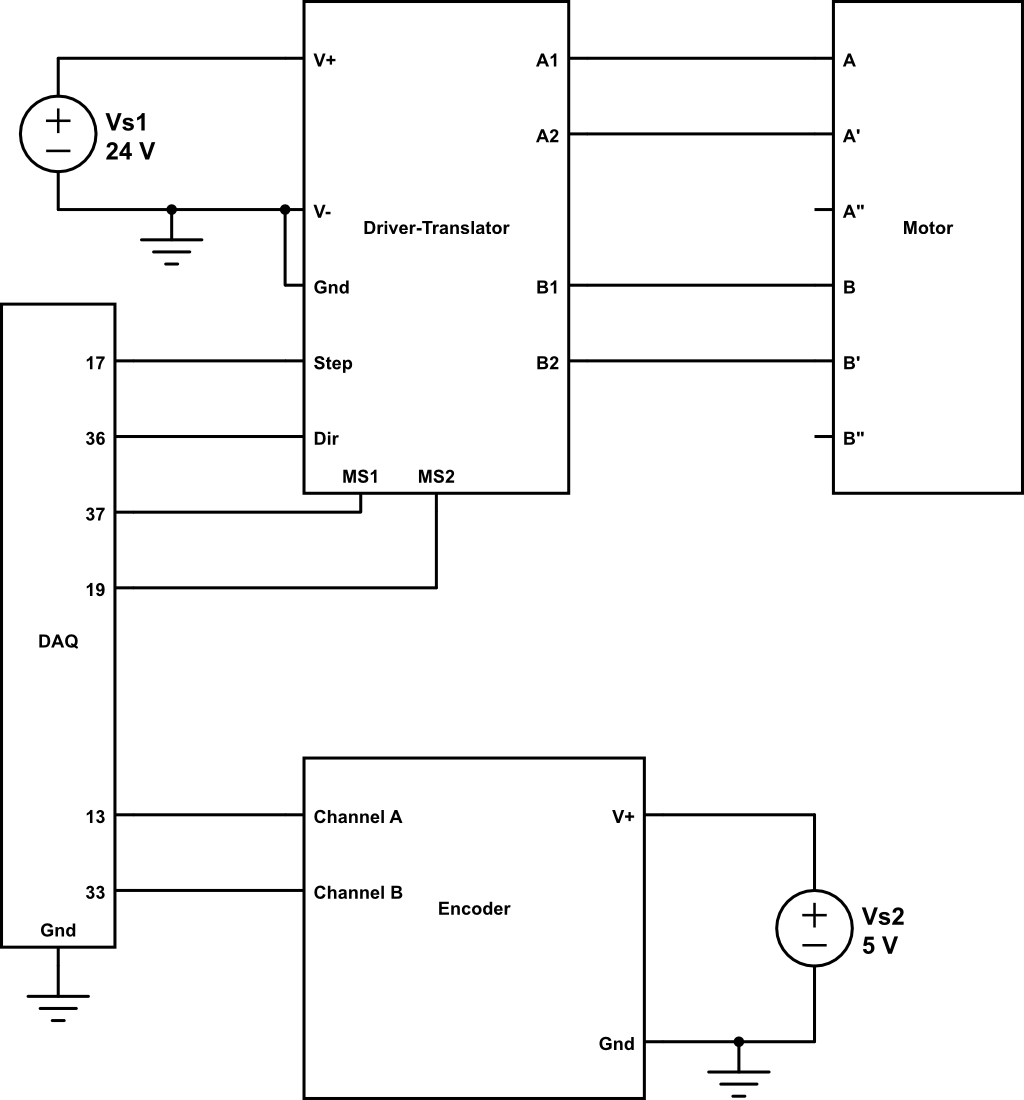
\includegraphics[width = 12cm]{lab5_main.png}
\caption{System level connection diagram. \xxx{Note all grounds are common}}
\label{q1_a}
\end{center}
\end{figure}

\subsection*{b.}
\begin{figure}[htb]
\begin{center}
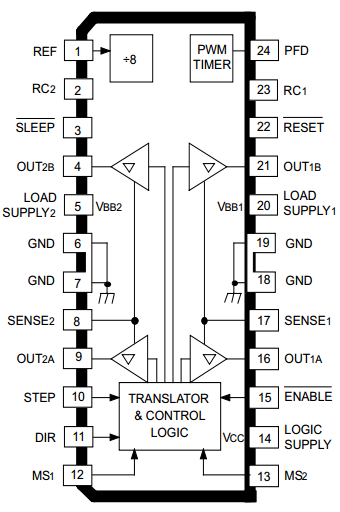
\includegraphics[width = 5cm]{A3967_pinout.png}
\caption{Pinout diagram of the A3967 chip.}
\label{q1_b}
\end{center}
\end{figure}

\begin{figure}[htb]
\begin{center}
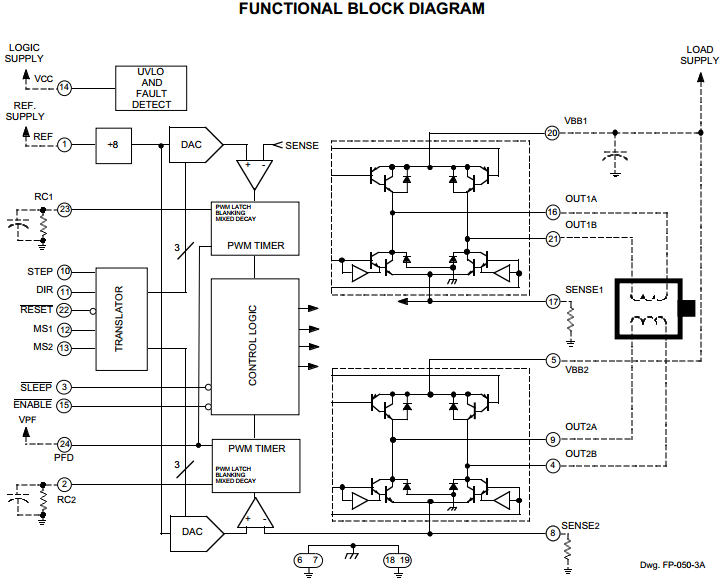
\includegraphics[width = 14cm]{A3967_functionalDiagram.png}
\caption{Functional diagram of the A3967 chip.}
\label{q1_b2}
\end{center}
\end{figure}

\subsubsection*{Pin1 - REF}
The \emph{REF} pin of the A3967 chip takes set the reference voltage for the logic circuit $V_{REF}$. It works in tandem with the senseristor to control the magnitude of the H-bridge current in the following manner:
\begin{itemize}
\item At $V_{REF} = 5$V max current will be 833mA.
\item At $V_{REF} = 3.3$V max current will be 550mA.
\item At $V_{REF} = 1$V max current will be 166mA.
\end{itemize}

From the functional diagram (figure \ref{q1_b2}), we see that $V_{REF}$ is fed into a DAC which is then fed to a comparator which then controls the PWM output, which in turn controls the current.\\

This input does not strictly require a dedicated external circuit, but the EasyDriver does provide a voltage divider circuit which is adjustable using a potentiometer thereby allowing us to \emph{tune} $V_{REF}$. 

\subsubsection*{Pin2 - RC2, Pin23 - RC1}
RC1 and RC2 control the fixed off-time for bridge 1 and bridge 2 respectively. Fixed off-time current regulation sets the current-decay modes of the H-bridges (slow, fast, or mixed).  The \emph{correct} current-decay control scheme can result in reduced audible motor noise, increased step accuracy, and reduced power dissipation.\\

According to the data sheet, the internal PWM current-control circuitry uses a one shot control scheme to regulate the time that the driver remains off.  The one shot off-time, $t_{off}$ , is determined by the selection of an external resistor ($R_T$) and capacitor($C_T$) connected from the $RC$ timing terminal to the ground. The off-time, over a range of values of $C_T = 470 pF$ to $1500 pF$ and $R_T = 12 k\Omega$ to $100 k\Omega$ is approximated by:
$$t_{off} = R_T C_T$$

The EasyDriver uses $R_T = 20k\Omega$ and $C_T = 680 pF$, hence $t_{off} = 0.0000136$s.\\

\subsubsection*{Pin3 - $\overline{\text{SLEEP}}$}
This terminal allows us to minimize power consumption when not in use. It works by disabling most of the internal circuitry and switching off the outputs of the chip. It is an active-low terminal, meaning that for normal operation a 1-logic command/high voltage signal needs to be sent to it, while in order to set the system to sleep, a 0-logic command/low voltage signal needs to be sent instead. When starting up from a sleep command, the device will return to its default/home position.\\

The EasyDriver provides a pull up resistor in series with this terminal to ensure it doesn't load the circuit it is connected to and also to prevent currents from flowing through it. Additionally, the terminal is set high by default which in turn can be toggled off by an external controller.


\subsubsection*{Pin4 - OUT2B, Pin9 - OUT2A, Pin16 - OUT1A, Pin21 - OUT1B}
These pins are the outputs of the H-bridge. As seen in the functional block diagram (figure \ref{q1_b2}), OUT-\emph{x}-A and OUT-\emph{x}-B represent the outputs of H-bridge \emph{x} and together complete the circuit of the respective phase of the motor.\\

The EasyDriver provides pin-outs for these terminals through jumper 3 (JP3).

\subsubsection*{Pin5 - LOAD SUPPLY2, Pin17 - LOAD SUPPLY1}
These pins provide the input power for the H-bridge to supply the motors. The data-sheet of the A3967 chip suggests that the supply voltage should be decoupled with an electrolytic capacitor ($>$47 $\mu$F is recommended). This decoupling is not provided in the EasyDriver PCB.\\


The decoupling capacitors would provide isolation from the supply sources noise as well as provide temporary boosting-effects if the load changes suddenly. The EasyDriver circuit assumes that the supply-source can react instantaneously and is relatively noise free.


\subsubsection*{Pin6 - GND, Pin7 - GND, Pin18 - GND, Pin19 - GND}
Connects various elements of the chip to the ground. The EasyDriver circuit takes care of this internally.

\subsubsection*{Pin8 - SENSE2, Pin17 - SENSE1}
The sense-terminals are connected to senseristors which measure the current flowing across them in order to control the output of the H-bridge. It forms a feed-back loop by acting as a \emph{sensor}. The EasyDriver PCB has 2 external sense-resistors of $0.75\Omega$, one for each H-bridge.

\subsubsection*{Pin10 - STEP}
The Step-terminal is an edge detector that operates on negative-to-positive changes in logic. On detecting such a transition, the  translator is told to advance the motor by one increment. Note that the input to the DACs and the direction of rotation are controlled by the translator itself, while the size of the increment is determined by the state of MS1  and MS2.\\

The EasyDriver provides direct access to this terminal through jumper 2 (JP2) and no external circuitry is required. A pull up resistor could be used just to be safe though.

\subsubsection*{Pin11 - DIR}
This pin determines the direction of rotation of the motor. The physical wiring of the motor decides which way the motor will actually rotate, however knowing that, this pin lets the user switch the direction digitally. The EasyDriver PCB allows for direct access of this pin through jumper 2 (JP2). The control logic for this pin is level dependent. Like the step control pin, a  pull up resistor could be used just to be safe.\\

\subsubsection*{Pin12 - MS1, Pin13 - MS2}
MS1 and MS2 together determine the size of an incremental step when a step command is given They are binary control variables with MS2 as the most significant bit and MS1 as the least significant bit. The corresponding results can be found in table \ref{q1_b3}.\\

\begin{table}[htb]
\begin{center}
    \begin{tabular}{|c|c|c|}
        \hline
        MS2 & MS1  & Increment Size          \\ \hline
        0   & 0    & Full step (2 phase) \\ 
        0   & 1    & Half step           \\ 
        1   & 0    & Quarter step        \\ 
        1   & 1    & Eighth step         \\
        \hline
    \end{tabular}
\caption{MS1 - MS2 based increment size determination.}
\label{q1_b3}
\end{center}
\end{table}

The EasyDriver puts a 10K buffer resistance before the MS1 and MS2 pins to increase the overall impedance of the pin and keeps both of them at a logic level of 1 by default (when unconnected) thereby resulting in the motor always taking 1/8$^{th}$ steps. An external controller can drop the voltages by forcing a drop to the terminals.

\subsubsection*{Pin14 - LOGIC SUPPLY}
The logic supply voltage, $V_{CC}$  can be set from $3.0$V up to $5.5$V \footnote{Subject to an absolute maximum of 7.0V}. On start-up if the logic supply is significantly below rated values, the system will go into its Under Voltage Lock Out (UVLO) mode where it switches off itself, thereby preemptively preventing damage.\\

The EasyDriver circuit provides a direct connection to $V_{CC}$ for this terminal. It is important to provide regulated voltage to this pin.

\subsubsection*{Pin15 - $\overline{\text{ENABLE}}$}
The Enable pin enables or disables the outputs. It is an active-low pin meaning that a logic-low should be sent in order to enable the chip. It is important to note however that the inputs to the translator (Step, Dir, MS1 , MS2) are all active independent of the Enable input state.\\

The EasyDriver PCB pulls the Enable pin down to the ground potential by default.



\subsubsection*{Pin22 - $\overline{\text{RESET}}$}
The Reset pin, as its name implies, resets the chip to its default operating points. It is an active-low pin meaning that a logic-low would reset the chip. When the chip is reset, the translator sets the DACs and phase current polarity to their initial home state, and sets the current regulator for both phases to mixed-decay mode. This simulates turning the chip off and then on again and it is useful while locally calibrating the chip back to its default home position to prevent errors from accumulating.\\

By default the EasyDriver sets this pin high, there by preventing reset. An external control circuit would have to pull it down to ground potential manually.

\subsubsection*{Pin24 - PFD}
The percentage fast decay controls the rate at which the current decays in the H-bridge. When an input signal command lowers the output current from the previous step, it switches the output current decay to slow, fast, or mixed-decay depending on the voltage level at the PFD terminal and the setting of the RC terminals. If the voltage is greater than 0.6$V_{CC}$ then slow-decay mode is selected.  If the voltage is less than 0.21$V_{CC}$ then fast-decay mode is selected.  Mixed decay is between these two levels and works by initially allowing for a steep current drop and then switching to a gradual drop.\\

The EasyDriver pcb has a 10k$\Omega$ attached to the pin by default and has a pin-out that enables us to attach an external resistor. 

\clearpage

\subsection*{c.}
\begin{figure}[htb]
\begin{center}
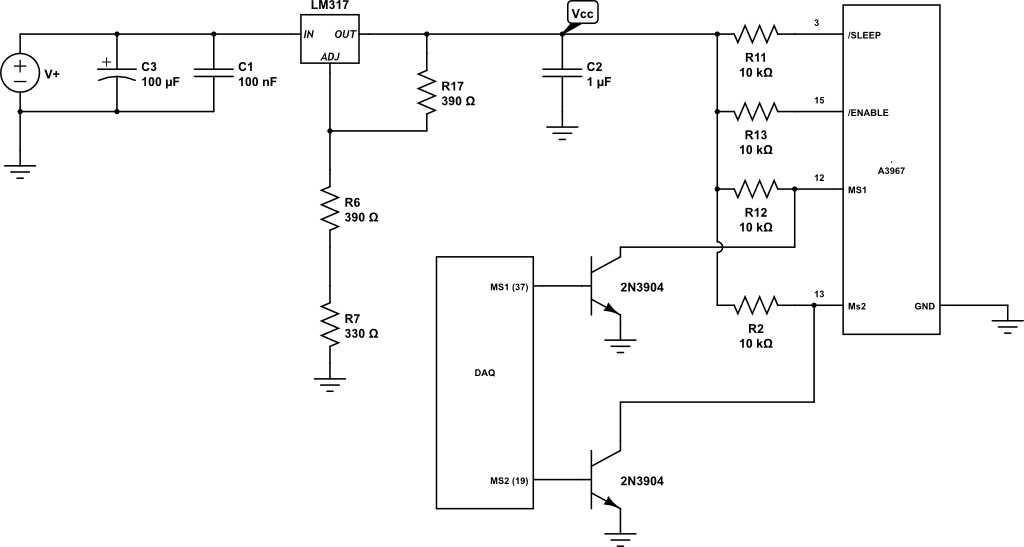
\includegraphics[width = 18cm]{lab5_q1_c.png}
\caption{Ideal Sleep, Enable, MS1 and MS2 pins connection diagram. \emph{Note: all grounds are common.}}
\label{q1_c}
\end{center}
\end{figure}

Figure \ref{q1_c} shows the ideal connection diagrams for the EasyDriver PCB along with some of the default connections already made on the board. The Sleep and Enable pins are low-enable pins. As we do not explicitly need to control them, we leave them in their default connection - with the EasyDriver pulling them up to $V_{cc}$.\\

$V_{cc}$ is generated by passing the main supply voltage through an LM317 voltage regulator that provides a relatively clean and stable 5V \footnote{Or 3.3V depending on the settings.}. This $V_{cc}$ is then used by the EasyDriver circuit to pull up pins as required. We use a 10$k\Omega$ resistor in series with the pin to act as a buffer resistor and so that if an external circuit is used to ground the pin, $V_{cc}$ is not connected to the ground directly.\\

For MS1 and MS2, we wish to control their states. By default the EasyDriver circuit pulls MS1 and MS2 up to $V_{cc}$. Ideally, to pull them to the ground potential we should use a decoupling transistor circuit as shown in figure \ref{q1_c}. This would then require the MS1 and MS2 control logic to be inverted as a high output would power the transistors to bring the pin potential to the ground. This design would electrically isolate the DAQ from the circuits.\\

 However, in our actual implementation, we connected the pin directly to the DAQ. This works as we have high a quality DAQ that can handle small circulating currents if they do arise\footnote{Due to mismatches in voltages.}.\\

The only change from default we incorporated was connecting MS1 and MS2. this was done to control the step size. 


\subsection*{d.}
We provided the 5V supply to our optical encoder from our external power source, the T60c switching power supply. Doing so has the following advantage:
\begin{itemize}
\item It provides a cleaner 5V - The circuitry on board the main power supply has more sophisticated circuitry than the LM741 regulator.

\item It has better cooling - The T60c is designed for high power output and as such is equipped for cooling.

\item Loading effects of the motor are not seen - if the motor draws a lot of power, its effects would be seen across the output of the voltage regulator. By decoupling the encoder power source from the motor driver, we can provide power irrespective of the power demands of the motor.
\end{itemize}

However it does also have the following disadvantages:
\begin{itemize}
\item 5V source could be contaminated with 60Hz noise - the T60 takes in 60Hz AC supply which could cause electromagnetic interference in the 5V supply.

\item The system becomes more spread out - using the 5V supply of the EasyDriver provides a more compact solution which helps us treat the system like a black box. Choosing the T60c would mean more wires come out of the system and hence more cabling costs.

\end{itemize}

Given the advantages and disadvantages, we chose the more reliable choice as we are only building a stationary prototype. Hence we can ignore any space constraints.


\section{LabView Implementation}
Figures \ref{q2_1} and \ref{q2_2} show the front panel and block diagram, respectively, of the LabView VI created to meet the requirements in the Lab 5 Instructions, as well as additional inputs and outputs for debugging. The front panel includes inputs for the user to select the mode (velocity vs. position), direction of rotation, step size, and input value with options for type of units (i.e. position as number of degrees or number of steps). Additionally, there is an overall power button (labeled "GO") and an option to save the encoder data using the "Write to Measurement File" block. In practice the data saving option was rarely used as it tended to slow down the simulation loop when set to high frequencies (over about 200 Hz).\\

The main output on the front panel is the "Motor Angle" waveform chart which displays the angular displacement obtained from the encoder via quadrature decoding. There is also a waveform chart for angular velocity which is only used for steady-state estimations for debugging because the filter used creates a significant delay. More accurate velocity values were obtained by exporting the displacement data and fitting lines to calculate slope. Additional debugging outputs consist of the "sum" indicator (which displays the current value of the edge counter), and LEDs for each of the outputs to the motor driver.     \\


\begin{figure}[h]
\begin{center}
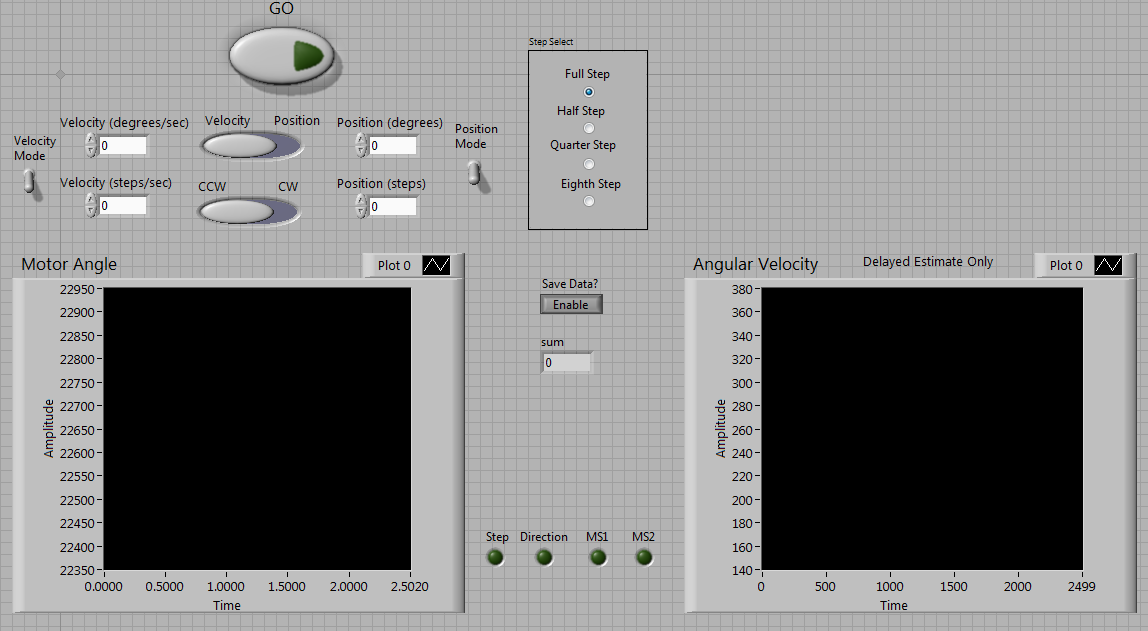
\includegraphics[width = 18cm]{VIFrontPanel.png}
\caption{Front panel of LabView VI.}
\label{q2_1}
\end{center}
\end{figure}

\begin{figure}[h]
\begin{center}
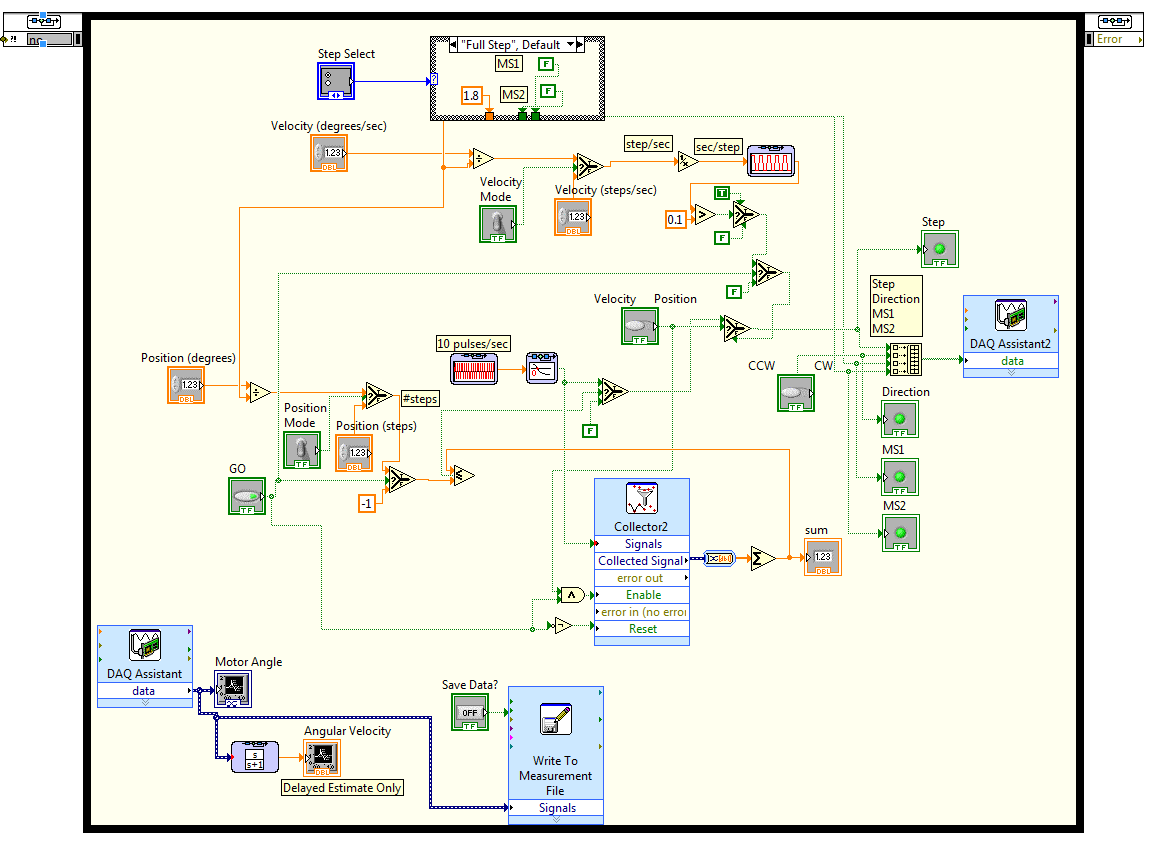
\includegraphics[width = 18cm]{VIBlockDiagram.png}
\caption{Block diagram of LabView VI.}
\label{q2_2}
\end{center}
\end{figure}

The VI uses a \emph{control \& simulation} loop running at 1000 Hz. At the top of the block diagram in figure \ref{q2_2} is a radio button block connected to a case structure. This is the step size selector. Depending on the button selected by the user, a constant is output corresponding to the degrees per step for that step size, and booleans are output for MS1 and MS2 according to the settings given in table \ref{q1_b3}.\\

Below the case structure is the velocity control segment of the VI. Based on the user's desired velocity, unit type, and step size, the number of steps per second is calculated and used to set the period of a "Pulse Signal" block. A greater-than comparator is then used to convert the 1's and 0's of the pulse signal into a stream of true and false booleans. This stream is put into an array along with a boolean for the direction of rotation and booleans for MS1 and MS2. This array is then sent to a DAQ Assistant block, which sends the array elements to the motor driver. Smaller step sizes resulted in smoother operation, but were not achievable at high velocities. Therefore, we left the step size as selectable rather than setting a specific step size.\\

In the middle of the block diagram is the position control section. At all times, a pulse generator is running at 10 Hz (arbitrarily selected; this could be a user input). The pulse signal is shifted downwards so that a zero crossing block can be used to detect the rising edges of the signal. Every time a rising edge is detected, the zero crossing block sends out a true boolean. However, this value only reaches the output array if the user has selected position mode and has selected the GO button. To stop after the desired number of steps has been taken, the output of the zero crossing block is also sent to a "Collector" block, which stores the values like an array. Summing the values within the collector gives the number of steps that have been taken. However, the collector is only enabled when the user selects position mode and the GO button (this makes the VI run faster in velocity mode, allowing for higher velocities). Additionally, the collector continuously resets itself when GO is not selected. This allows for multiple runs, and prevents the always running pulse signal from storing edge counts when not desired. The user's desired displacement is converted to the number of steps required, and a less-than-or-equal-to comparator is used to stop the stream of pulses to the output when the edge count reaches the required number of steps.\\

At the bottom of the block diagram is the input from the encoder, which is not used for control feedback. A derivative and filter are used to display the angular velocity. However, there is a significant delay, so the velocity chart was only used for debugging at steady-state. A block to save the encoder data to a file is provided, but was rarely used as it had a significant negative impact on the speed of the simulation loop.   \\


Additional VI's were created to fulfill the specialized objectives of some of the laboratory questions.\\

\subsection*{LabView Difficulties}

Labview is not fundamentally well suited to the task of driving the stepper motor because of our limited ability to reconstruct output signals of different frequencies.  Even avoiding the use of slow control and simulation loops and resorting to just a while loop, LabView only has access to a clock with a resolution of just $1$ ms.  This means that as we approach the maximum frequency that this timer will allow us to reconstruct, $500$ Hz we run into quantization issues illustrated in table \ref{Q2_T2}, which prevent us from outputting arbitrary frequencies.  This problem is less important for low frequencies, but it is still present.  

\begin{table}
\begin{center}
    \begin{tabular}{|c|c|c|c|c|c|c|c|c|c|c|}
        \hline
        Signal    & 1 & 2 & 3 & 4 & 5 & 6 & 7 & 8 & 9 & 10 \\ \hline
        500 Hz    & 1 & 0 & 1 & 0 & 1 & 0 & 1 & 0 & 1 & 0  \\ 
        333.33 Hz & 1 & 0 & 0 & 1 & 0 & 0 & 1 & 0 & 0 & 1  \\ 
        250 Hz    & 1 & 1 & 0 & 0 & 1 & 1 & 0 & 0 & 1 & 1  \\ 
        200 Hz    & 1 & 1 & 0 & 0 & 0 & 1 & 1 & 0 & 0 & 0  \\
        \hline
    \end{tabular}
\caption{LabView Frequency Discretization}
\label{Q2_T2}
\end{center}
\end{table}

We can physically illustrate this issue by commanding a linear velocity output from LabView.  If the velocity profile was linear, then we would expect a quadratic position output.  However, as shown in figure \ref{Q2_3} we see roughly linear regions in the position output, the last two of which are at $333.33 \, Hz$ and $500 \, Hz$ respectively. Indicating that we are indeed seeing quantized frequency outputs.

\begin{figure}[hbt]
\begin{center}
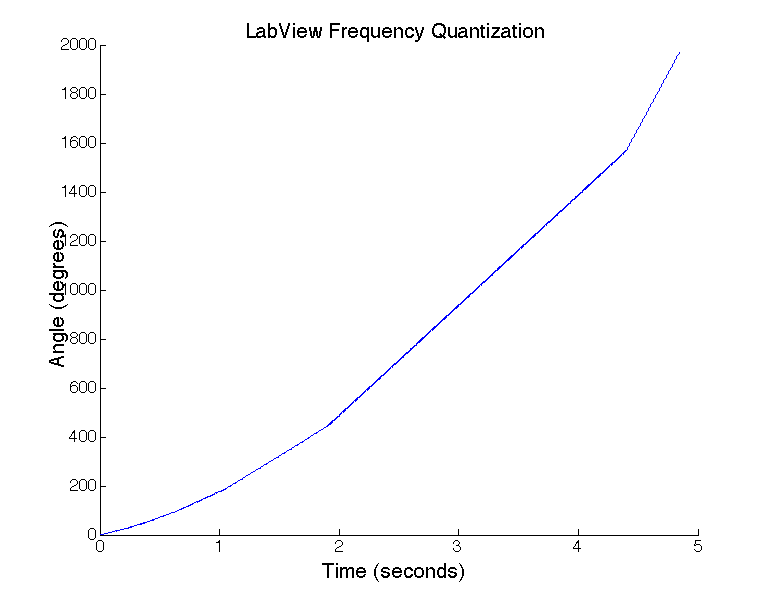
\includegraphics[width = 13cm]{frequencyQuantization.png}
\caption{Illustration of LabView Frequency Quantization}
\label{Q2_3}
\end{center}
\end{figure}

\clearpage

\section{Experimental Characterization}
\subsection*{a.}
Step response data was obtained using the previous VI at 1000 Hz in both the loaded and unloaded conditions, as well as in the clockwise and counter-clockwise directions. Even at LabView's max frequency the number of data points recorded of the motor's oscillations was not enough to generate a smooth curve on their own. Curve fitting was attempted, but had little effect (as shown in figure \ref{q3a_1}). Additionally, the relatively low resolution of the encoder made accurate measures of the amplitude of oscillations impossible. Figure \ref{q3a_1} shows one data set from our tests. After the initial overshoot, all of the oscillations have the same amplitude. This would make it appear that the system is undamped, when in reality, the encoder is not able to tell the difference between the oscillations. This quantization error had a significant impact on the estimations of overshoot, and therefore on the damping ratio ($\zeta$).\\

\begin{figure}[hbt]
\begin{center}
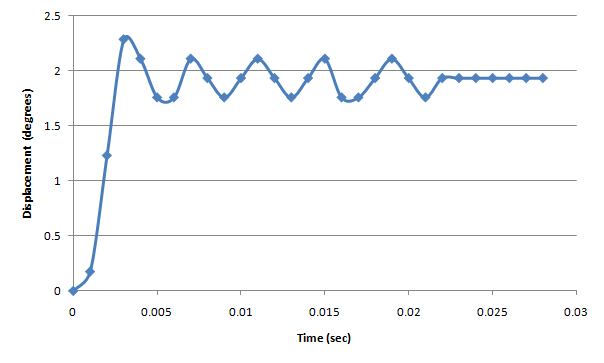
\includegraphics[width = 14cm]{StepResponse.png}
\caption{Step response of loaded stepper motor.}
\label{q3a_1}
\end{center}
\end{figure}

\subsubsection*{i}

Table \ref{q3ai_!} shows the average rise time and other parameters for both the loaded and unloaded conditions. The unloaded motor had a slightly smaller overshoot, leading to a larger damping ratio. However, this conflicts with the unloaded case having more oscillations before becoming steady. We found that the belt system had a significant amount of "springiness," which is likely affecting our results. Also, the steady-state error values are not very reliable due to the quantization of the encoder. It is possible that the motor stepped perfectly to 1.8$\circ$ (one full step), but if the encoder does not have a "tick" at that exact point, it would output the closest possible reading (in either direction depending on how the oscillations settle). This leads to an inaccurate estimation of steady-state error. \\


Table \ref{q3ai_@} shows the calculated frequency values and damping ratio for the loaded and unloaded conditions. The damping ratio was calculated using the percent overshoot. Because the overshoot is affected by the quantization error of the encoder, the damping ratio also has a large amount of error. Because the encoder tends to cut-off the peak of the overshoot, the damping ratios given here should be considered underestimates. The damped frequency was calculated from the peak-to-peak period of the oscillations, and the natural frequency was calculated using the damped frequency and the damping ratio.\\


\begin{table}[htb]
\begin{center}
    \begin{tabular}{|c|c|c|c|c|}
        \hline
        Condition & Rise Time (s)  & Overshoot (\%) & Oscillations (\#) &  Absolute Steady-State Error (degree)   \\ \hline
        Loaded   & 0.00267    & 19.512 & 7.5 &   0.065 \\ 
        Unloaded   & 0.00203    & 12.830 & 11 & 0.109         \\         
        \hline
    \end{tabular}
\caption{Average step-response parameters.}
\label{q3ai_!}
\end{center}
\end{table}

\begin{table}[htb]
\begin{center}
    \begin{tabular}{|c|c|c|c|c|c|}
        \hline
        Condition & $f _n$ (Hz)  & $\omega _n$ ($\frac{rad}{sec}$) & $f _d$ (Hz) &  $\omega _d$ ($\frac{rad}{sec}$) & Damping Ratio, $\zeta$   \\ \hline
        Loaded   & 295.495   & 1856.651 & 262.146 &  1647.110 & 0.4616\\ 
        Unloaded   & 330.474   & 2076.431 & 272.690 & 1713.361 & 0.5552         \\         
        \hline
    \end{tabular}
\caption{Average natural and damped frequency values.}
\label{q3ai_@}
\end{center}
\end{table}

The generic second order transfer function is given by equation \ref{q3ai_A} where K is the system gain based on the average steady-state error. Plugging in the calculated values for the loaded condition gives the result shown in equation \ref{q3ai_B} and in figure \ref{q3ai_1}. The figure shows that the transfer function is not a very good fit to the experimental data. First, the overshoot is not large enough, and the oscillations die out too fast. As mentioned previously, the quantization of the encoder leads to an overestimation of the damping ratio, so this behavior is not very surprising. Also the rise time is too short. This is likely caused in part because the model does not include the effect of the finite rise of the current and coulomb friction in the system. This can especially be seen in the shallower slope between the first two points on the experimental curve. By reducing the damping ratio until the overshoot was greater than the overshoot of the experimental data set by an amount equal to the encoder resolution (which also resulted in a new value for natural frequency because we had directly measured the damped frequency and then calculated the natural frequency using the damping ratio) we obtained the transfer function shown in equation \ref{q3ai_C} and in figure \ref{q3ai_2}. This fits the data much better, particularly the time of the first several peaks. However, the model still dies out much faster than the real system.\\

\begin{equation}
\label{q3ai_A}
T(s) = K \frac{\omega _n^2}{s^2 + 2\zeta \omega _n s + \omega _n^2}
\end{equation}

\begin{equation}
\label{q3ai_B}
T(s) = \frac{3322707.14}{s^2 + 1715.55 s + 3447149.22}
\end{equation}

\begin{figure}[hbt]
\begin{center}
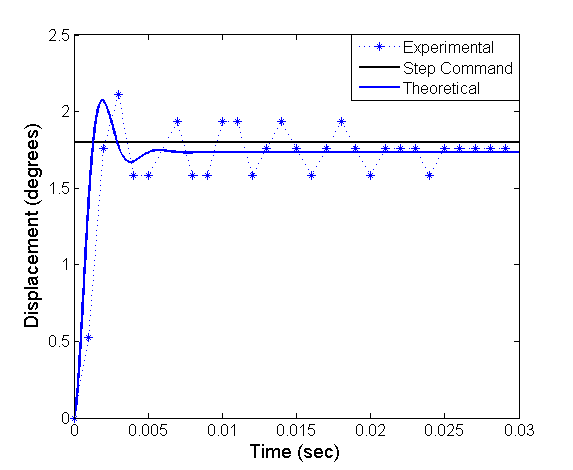
\includegraphics[width = 11cm]{LoadedStepUnFit.png}
\caption{Theoretical step response of loaded motor using calculated values.}
\label{q3ai_1}
\end{center}
\end{figure}

\begin{equation}
\label{q3ai_C}
T(s) = \frac{2956844.29}{s^2 + 1190.99 s + 3067584.07}
\end{equation}

\begin{figure}[hbt]
\begin{center}
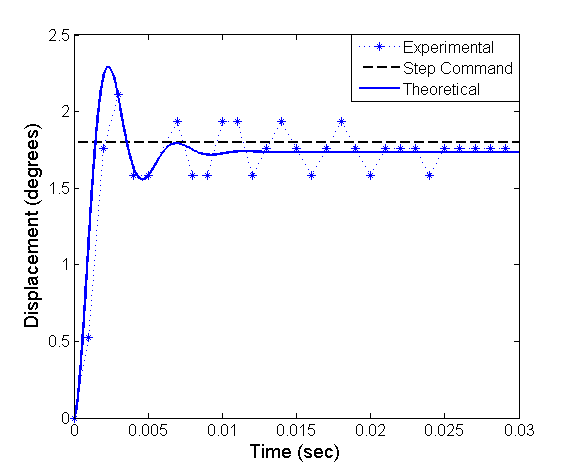
\includegraphics[width = 11cm]{LoadedStepFit.png}
\caption{Theoretical step response of loaded motor using fit values.}
\label{q3ai_2}
\end{center}
\end{figure}
\vspace{5mm}
The same procedure was performed for the unloaded condition. As before, the calculated values result in a poor fit with the experimental data (see equation \ref{q3ai_D} and figure \ref{q3ai_3})  due to the inaccurate damping ratio and unmodeled dynamics. Adjusting the damping ratio to account for the theoretical higher overshoot that the encoder cuts off gives the results shown in equation \ref{q3ai_E} and figure \ref{q3ai_4}. Again, this is a better fit, but the model still dies out much faster than the real system.\\

\begin{equation}
\label{q3ai_D}
T(s) = \frac{4050280.92}{s^2 + 2305.67 s + 4311561.54}
\end{equation}

\begin{figure}[hbt]
\begin{center}
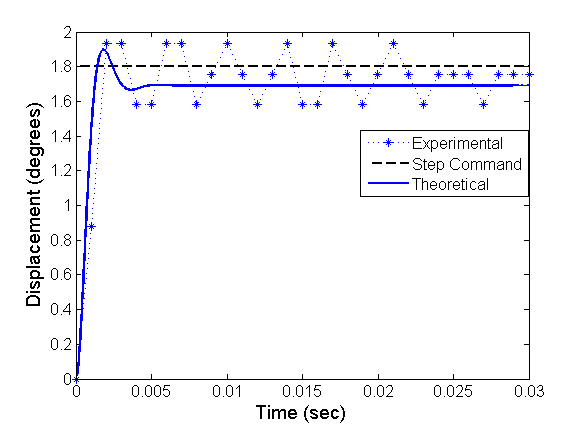
\includegraphics[width = 11cm]{UnloadedStepUnFit.png}
\caption{Theoretica vs empirical step response of unloaded motor using calculated values.}
\label{q3ai_3}
\end{center}
\end{figure}

\begin{equation}
\label{q3ai_E}
T(s) = \frac{3314951.55}{s^2 + 1540.38 s + 3528796.63}
\end{equation}

\begin{figure}[hbt]
\begin{center}
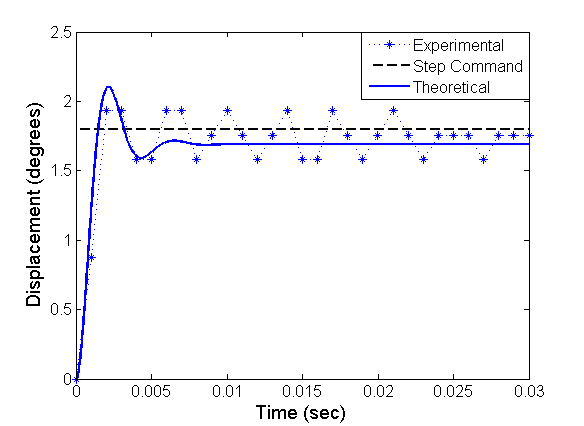
\includegraphics[width = 11cm]{UnloadedStepFit.png}
\caption{Theoretical vs empirical step response of unloaded motor using fit values.}
\label{q3ai_4}
\end{center}
\end{figure}

The rise time of the system is affected by a combination of the inertia of the rotor (and transmission in the loaded condition) and the finite rise time of the current. The addition of the load increases the rise time by over 25\%. Because the current cannot immediately jump to its max value, the motor torque starts low and increases as the current increases, increasing the rise time over the theoretical value. Viscous and coulomb friction also affect the rise time, particularly as the current/torque need time to increase to the point where the static friction can be overcome. However, the static friction in this system is not very large.\\

The overshoot is also affected by the inertia of the system, as the rotor/belt/pulley want to keep moving past the commanded position. The viscous and coulomb friction affect the overshoot as they act to slow the system, but the values are not significant, so their effect on damping the overshoot and oscillations is negligible (the springiness of the belt could have a large effect but is highly nonlinear and could contribute positively or negatively). A larger effect is provided by the magnetic stiffness. With the coils energized, the shaft is always pulled towards the stable equilibrium. This is what brings the motor shaft back towards the set point after it overshoots. Because the magnetic stiffness is dependent on the current from the driver, the finite decay and rise time in the chopper circuit affect the overshoot.\\

The oscillations of the motor shaft are affected very much like the overshoot. The inertia of the system is what keeps the oscillations moving, while the magnetic stiffness is what drives the shaft towards the set point. Viscous and coulomb friction act to damp out the oscillations, and the current rise/decay causes the magnetic stiffness to vary. Finally, the steady-state error is determined by the magnetic stiffness and external loads. The coils always try to pull the shaft into stable equilibrium while the only steady state load on the system is static friction.  The motor might have reached 0 steady state error, however the quantization error of the encoder means that our position reading could be slightly off.\\


\clearpage
\subsubsection*{ii}

Despite sweeping a variety of frequencies using a function generator we were unable to to cause the system to become unstable until we exceeded the pull-out frequency.  However, while the motor did remain stable, there was a noticeable decrease in response quality at some frequencies.  This was characterized by a highly under-damped response as shown in figure \ref{Q3_aii1} at resonance compared to the much more damped out response shown in figure \ref{Q3_aii2} away from resonance.\\


\begin{figure}[hbt]
\begin{center}
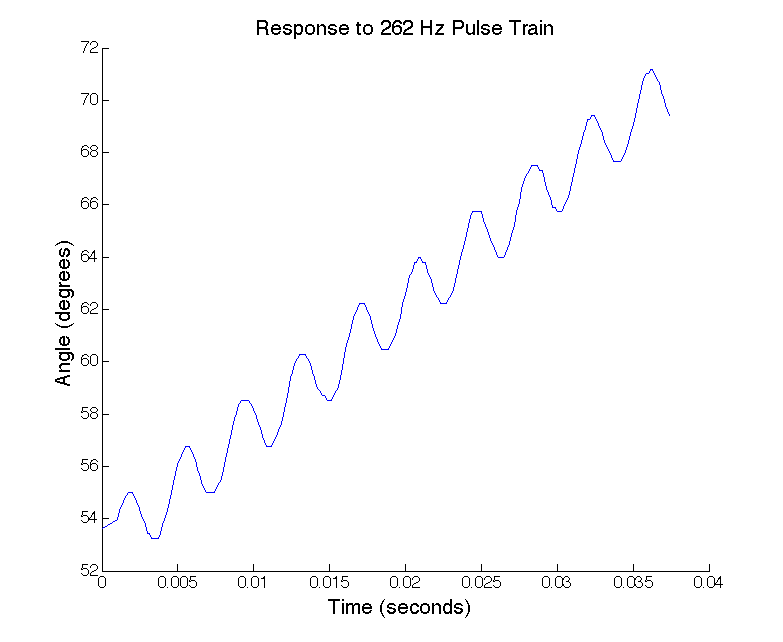
\includegraphics[width = 10cm]{262Hz_Response.png}
\caption{Undamped response at Resonance, Loaded, full-step, 262 Hz}
\label{Q3_aii1}
\end{center}
\end{figure}

\begin{figure}[hbt]
\begin{center}
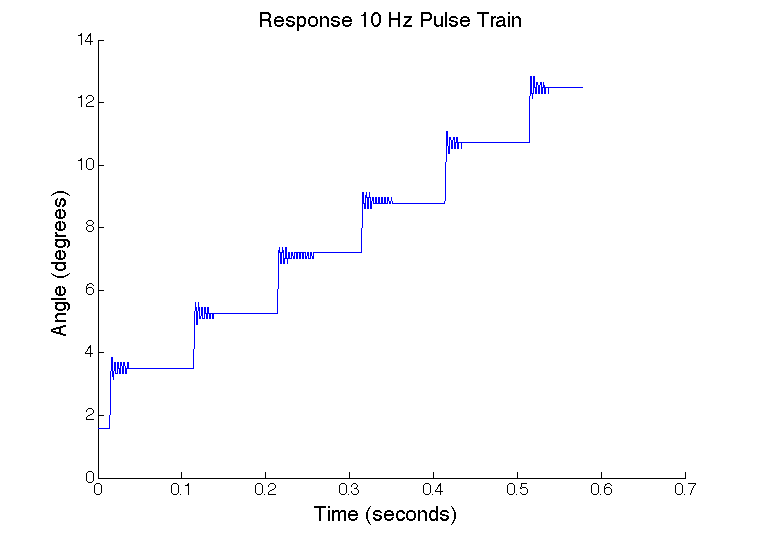
\includegraphics[width = 10cm]{10Hz_Response.png}
\caption{Damped response at away from Resonance, Loaded, full-step, 10 Hz}
\label{Q3_aii2}
\end{center}
\end{figure}

To quantify the response quality we constructed a metric where we measured the number of loop iterations for which the angle reported by the encoder was beyond 1 full step off from the commanded value.  This measure would be expected to perform poorly for high step rates, as the rise time would become large compared to the length of each step.  For low to intermediate frequencies this metric seemed to characterize the quality of response well enough.  We commanded full steps at rates between $25$ Hz to $600$ Hz at $25$ Hz intervals and measured this excursion fraction for the loaded and unloaded cases, as shown in figure \ref{q3aii}.\\


\begin{figure}[hbt]
\begin{center}
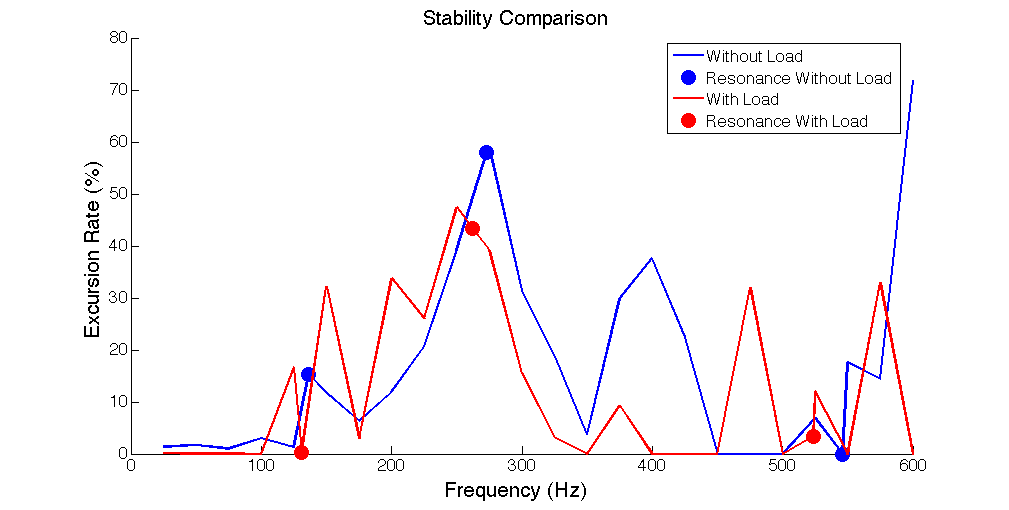
\includegraphics[width = 15cm]{ResonanceData.png}
\caption{Percentage of Time of Response differed from Commanded Angle by more than 1 full step.}
\label{q3aii}
\end{center}
\end{figure}

We also performed additional trials at the resonant frequency, half of that frequency, and double that frequency for the loaded and unloaded cases.  The data confirms our estimates of the natural frequencies with peaks in the expected regions.  However we also notice poor response at other frequencies as well interrupted by occasional frequencies that ran very smoothly. 

\clearpage

\subsection*{b.}

Pull-in speed is defined as the maximum step-rate command that may be issued to the stepper motor from rest such that the stepper motor remains synchronized with the pulse train.  Due to the frequency quantization issues caused by LabView, it was necessary to conduct these experiments using an external function generator.  

LabView was then used to record the number of pulses sent by the function generator and encoder pulses as shown in figures \ref{q3b_Front} and \ref{q3b_Back}.  The motor angle was again measured using quadrature decoding and outputs measurements in degrees.  The number of pulses were counted using the other counter input of the DAQ set to trigger on Rising edges.  The LabVi still had a control to set the direct, while the step mode was set using built in parameters.  The \emph{Measured Steps} field reports the number of steps that the stepper motor has gone through based on its current position and the angle covered by each step.  The \emph{Commanded Steps} field reports the number of steps reported by the counter, and \emph{Step Error} is their difference.  \emph{Fault} reports when the step error exceeds 1, and \emph{Number Faults} records the number of loop iterations that \emph{Fault} has been true while \emph{Total} is simply the number of loop iterations that have elapsed. The vi is configured to terminate once a set number of iterations have elapsed, but this figure was not always used.  

Knowing the angle per full step, we can then directly compare the commanded position with the actual position.  However this comparison is very difficult while the system is still in motion when we wish to determine the pull-in speed, because we do not expect the two values to diverge, even when we have lost synchronization.  Instead we expect for values just above the pull-in speed, but below the pull-out speed, that there will be some approximately constant offset between the two equal to the number of steps lost when starting up.   But this offset is difficult to see while the system is in motion, especially for small numbers of missing steps.\\  

To deal with this issue, the offset was evaluated after the system was brought to a complete stop. For each trial, with the stepper motor at rest, the LabView VI was started.  Then the function generator was activated outputting a square wave of some frequency.  The pulses from the function generator and the encoder were recorded and the function generator stopped.  Then the final commanded position was compared with the actual stepper motor angle.  If these values differed by at least 1 step, then we say that the speed was above the pull-in speed of the system.  In practice, the difference was always either very small, due to encoder discretization, or off by integer steps, again, up to encoder discretization.  After some testing the pull-in frequencies for the full step setting were determined and are shown in table \ref{q3b_table1}.


\begin{figure}[htb]
\begin{center}
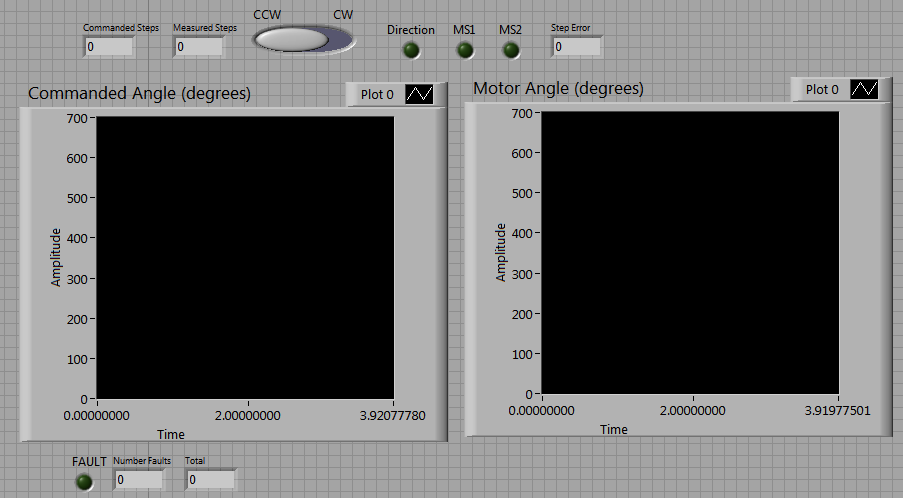
\includegraphics[width = 13cm]{ExternalSourceFront.png}
\caption{VI Front panel used for Pull-In and Pull-out torque estimates}
\label{q3b_Front}
\end{center}
\end{figure}

\begin{figure}[htb]
\begin{center}
\includegraphics[width = 13cm]{ExternalSourceBack.png}
\caption{VI used for Pull-In and Pull-out torque estimates}
\label{q3b_Back}
\end{center}
\end{figure}

\begin{table}[htb]
\begin{center}
    \begin{tabular}{|c|c|c|}
        \hline
        ~                    & Unloaded & Loaded \\ \hline
        Pull-In Frequency $(Hz)$ & 545        & 469      \\
	Pull-In Speed $(\sfrac{deg}{s})$ & 981 & 844.2 \\
        \hline
    \end{tabular}
\caption{Pull-in Frequencies and speeds found for full step in the loaded and unloaded cases.}
\label{q3b_table1}
\end{center}
\end{table}

We used the same VI as shown in figures \ref{q3b_Front} and \ref{q3b_Back} to determine the pull-out speeds for the loaded and unloaded cases.  Again we monitored the recorded number of pulses sent to the stepper motor and the current position of the stepper motor measured in steps.   When these two values diverged, we knew that the stepper motor had lost synchronization.  The pull-out frequency was determined simply by using the function generator and manually ramping the output frequency up until the motor lost synchronism.  The frequencies determined by these tests for the loaded and unloaded cases are shown in table \ref{q3b_table2}.

\begin{table}[htb]
\begin{center}
    \begin{tabular}{|c|c|c|}
        \hline
        ~                       & Unloaded & Loaded \\ \hline
        Pull-Out Frequency (Hz) & 1088.6   & 1077.9 \\
	Pull-Out Speed $(\sfrac{deg}{s})$ & 1959.5 & 1940.2 \\
        \hline
    \end{tabular}
\caption{Pull-out frequencies for loaded and unloaded cases}
\label{q3b_table2}
\end{center}
\end{table}

It is quite clear from these two experiments that the pull-out speed is greater than the pull-in speed.  This is simply because of the dynamics of the rotor.  The rotor has some inertia and to accelerate it at some rate requires a certain amount of torque.  To achieve some stepping rate from rest, we must accelerate to that angular velocity in the period of a single step.   Even if we ignore the additional electrical dynamics which mean that coil current has some non-zero rise time, the torque exerted by the stepper motor is some finite amount.  This imposes an upper limit on the changes in angular velocity that can be made while keeping the rotor synchronized with the command pulse train.  The maximum speed that can be commanded from rest is known as the pull-in speed.

$$ \sum \tau = J \dot{\omega} = \tau_m - \tau_{Load} \hspace{1cm} \dot{\omega} \approx \frac{\Delta \theta}{(\Delta t)^2} \hspace{1cm} \Delta t = \frac{1}{f_{command}}$$

$$ f_{command \, max} \approx \sqrt{\frac{J \, \Delta \theta}{\tau_{m} - \tau_{Load}}} $$

Effectively some motor torque is being used to accelerate the rotor while the rest is working against the load.  So for large accelerations, less of the motor torque is available to overcome the load torque.  However if accelerations are kept sufficiently small, then all of the motor torque is available to overcome load torque, allowing the rotor to reach higher angular velocities while remaining synchronized with the command pulse train than it could in a single step change in angular velocity.  

\clearpage

\section{Motion Control}
\subsection*{a.}

\begin{figure}[h!]
\begin{center}
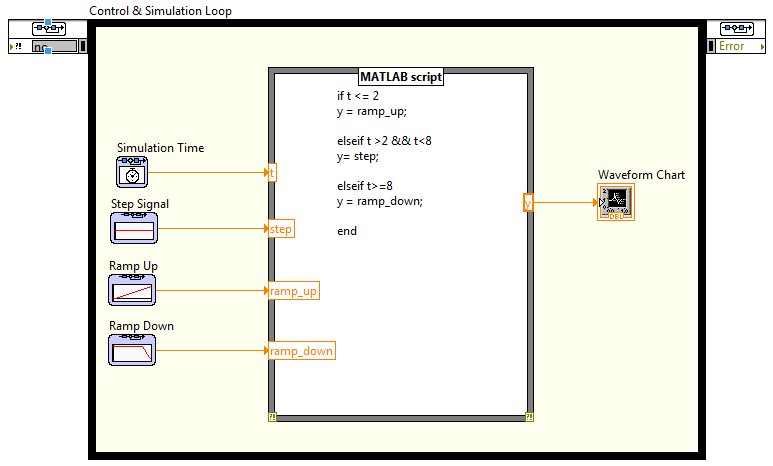
\includegraphics[width=16cm]{Q4_CommandGeneration_VI.png}
\caption{Trapezoidal Velocity Profile Generation- Example VI} \label{tex}
\label{fig:q4_1}
\end{center}
\end{figure}

Based on the specified constraints of velocity profile, the velocity command would be a function of time. Instead of the previous numeric input of velocity control, the ramp and step signals were combined together as a velocity command to generate the desired trapezoidal profile. As shown in Figure~\ref{fig:q4_1}, the step signal was used for the constant speed region with all values equal to 180, and two ramp signals were used to create the acceleration and deceleration regions with +90 and -90 acceleration [deg/s$^{2}$], respectively. Next, the matlab code switched the correct signal to the output y in the right time: (1) 0-2 sec: the rising ramp; (2) 2-8 sec: the step input; (3) 8-10 sec: the descending ramp. The output y was simply connected to the velocity input in the block diagram of main VI (see Figure 5), so that the desired function of velocity commands could be achieved. Figure~\ref{fig:q4_2} plots the resulting trapezoidal velocity profile, which satisfies all the requirements without considering the rest of control loop.\\

However, the actual velocity and displacement profiles from the experimental results seemed far different from the expected profiles (see Figure~\ref{fig:q4_3} and~\ref{fig:q4_4}). Despite the total displacement being close to 1440deg, the velocity seemed to changed disorderly with respect to the time frame. One possible reason is that the pulse generator is unable to be synchronized with the reference command; some pulses may be missed or their frequencies could be incorrect at some certain time. Furthermore, the computation time by the matlab code or other logic control may lead to time delay since the step size cannot be too small in order to synchronize with real time. Additionally, the ideal trapezoidal profile is based on the assumption of unlimited jerk, so that the real behavior of the stepper motor might deviate what we expect.\\

\begin{figure}[h!]
\begin{center}
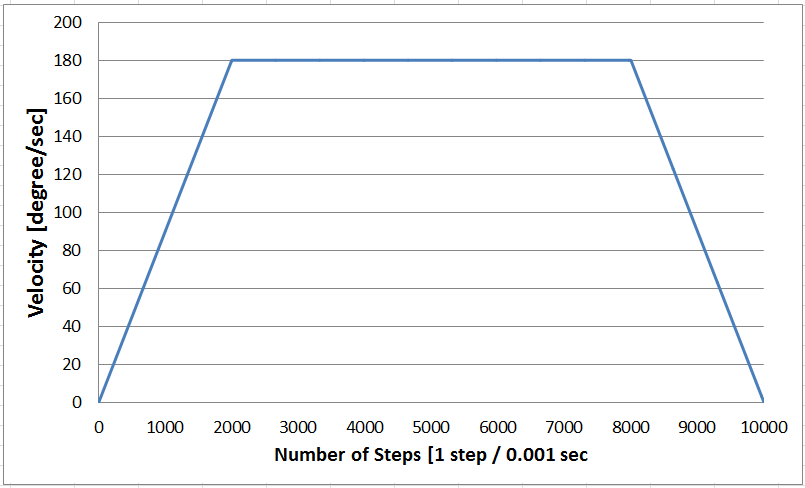
\includegraphics[width=12cm]{Q4_CommandGeneration.png}
\caption{Trapezoidal Velocity Command} \label{tex}
\label{fig:q4_2}
\end{center}
\end{figure}

\begin{figure}[b!]
\begin{center}
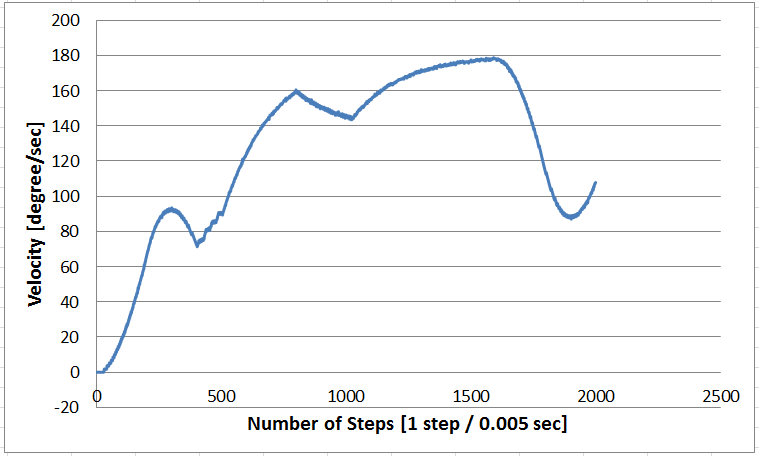
\includegraphics[width=12cm]{Q4_Trapezoid_Velocity_Fail.png}
\caption{Filtered Velocity Profile} \label{tex}
\label{fig:q4_3}
\end{center}
\end{figure}
  
\begin{figure}[h!]
\begin{center}
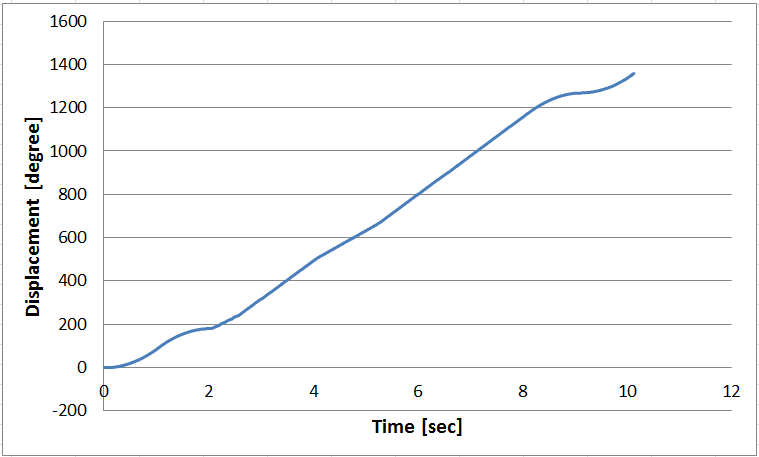
\includegraphics[width=12cm]{Q4_Trapezoid_Displacement_Fail.png}
\caption{Actual Displacement Profile} \label{tex}
\label{fig:q4_4}
\end{center}
\end{figure}

%%%%%%%%%%%%%%%%%%%%%%
% here is John's new stuff with the alternate Matlab stuff

\clearpage

We devised an alternative LabView Vi to attempt to fulfill the specification shown in figures \ref{Q4a_Alt1} and \ref{Q4a_Alt2}.  By avoiding the use of computationally expensive "Blue Blocks" where possible and sticking with an inexpensive while loop, we hoped to achieve as much performance as possible.  This version generates linear velocity profiles by sampling a frequency after the previous half period has elapsed and using this sampled frequency to compute a new period to wait for.  This behavior is approximately correct for high frequencies but diverges for low frequencies from the intended profile.  For example, a command of $0 \, Hz$ with a slope of $1 \, Hz$ per second, we would expect a pulse roughly at the 1 second mark, however, this version will wait infinitely long before giving any pulses.  

The block diagram in figure \ref{Q4a_Alt2} has several key features.  Starting in the lower right are the digital outputs with the \emph{MS1} and \emph{MS2} pins configured to false, while the direction is tied to a toggle.  Immediately to the left is a small loop that simply switches between true and false when given a pulse.  The upper right segment to the right of the multiplication by $0.5$ consists of a counter and a timer.  The left most loop in this cluster keeps track of the previously given period and when it is altered sends pulses to the timer circuit below and the counter to the right to reset to zero.  This counter and the current period are compared to the timer value to determine when to send a pulse.  The multiplication by 0.5 on this input ensures that it will pulse every half period.  The \emph{AND} which takes the output from the system ensures that the current period will only be updated at every half period.  The cluster to the right is used to toggle between a constant frequency and a linear frequency profile.  The linear frequency profile is obtained through the use of a timer and the given frequency slope.  The far right cluster computes the switching times between different parts of the trapezoid going from a linear increase in slope, to a constant slope and decreasing slope before finally turning off all output. 

This bug was addressed by starting at a non-zero frequency, which results in the actual position getting ahead of the desired position, as shown in figures \ref{Q4a_Alt3}, \ref{Q4a_Alt4}, and \ref{Q4a_Alt7}.  This lead to a profile that was not quite correct but was relatively close and most importantly did get to the final position.  We do see in figure \ref{Q4a_Alt6} that the stepper motor easily remains synchronized with these commands.  This bug could have potentially been eliminated by including a look ahead of some sort in the profile, but this look ahead would have a rather complicated dependence on the value of the frequency at this look ahead position.  Also considering that LabView would be unable to reproduce frequencies significantly higher with any degree of accuracy anyway, we switched over to using a function generator to drive the stepper motor.

\begin{figure}
\begin{center}
\includegraphics[width = 13cm]{trapezoidLabViewFront.png}
\caption{Alternative Trapezoid Velocity Profile LabView Front Panel}
\label{Q4a_Alt1}
\end{center}
\end{figure}

\begin{figure}
\begin{center}
\includegraphics[width = 16cm]{trapezoidLabViewBlock.png}
\caption{Alternative Trapezoid Velocity Profile LabView Block Diagram}
\label{Q4a_Alt2}
\end{center}
\end{figure}

\begin{figure}
\begin{center}
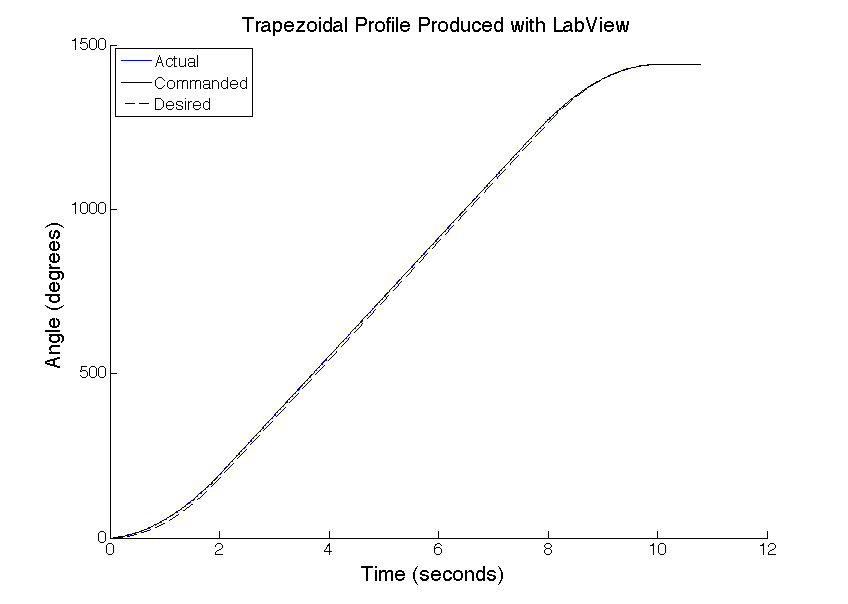
\includegraphics[width = 12cm]{labViewProfile.png}
\caption{Alternative trapezoidal Velocity Profile}
\label{Q4a_Alt3}
\end{center}
\end{figure}

\begin{figure}
\begin{center}
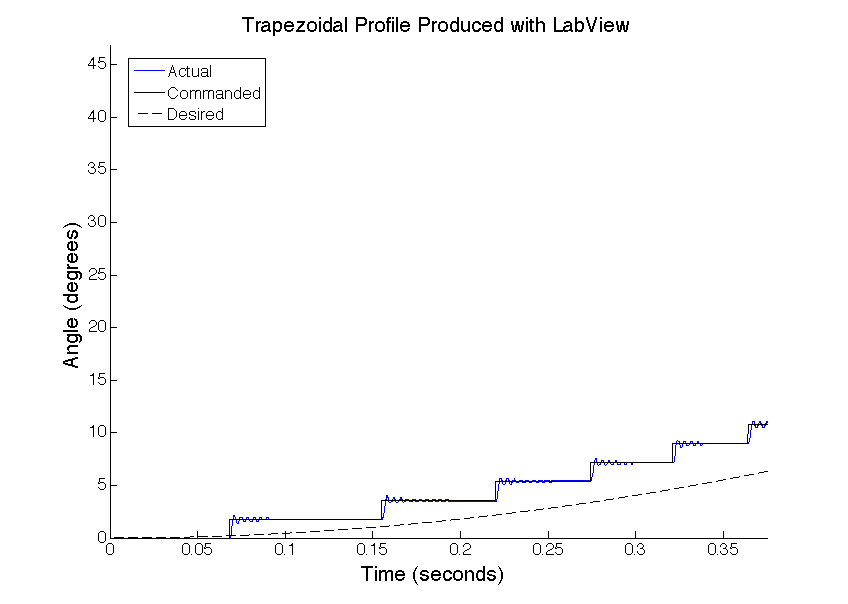
\includegraphics[width = 12cm]{labViewProfile_Detail2.png}
\caption{Alternative Trapezoid Velocity Profile}
\label{Q4a_Alt4}
\end{center}
\end{figure}

\begin{figure}
\begin{center}
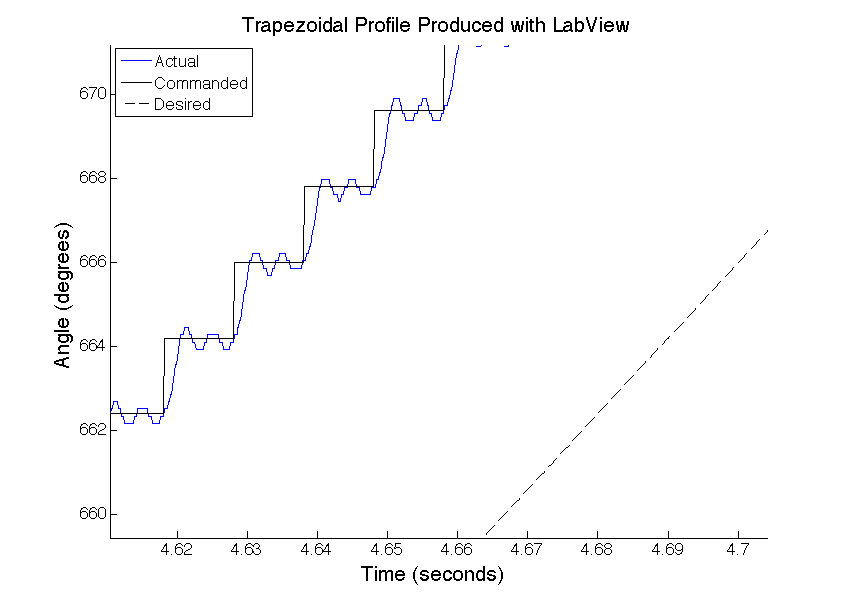
\includegraphics[width = 12cm]{labViewProfile_Detail1.png}
\caption{Alternative Trapezoid Velocity Profile}
\label{Q4a_Alt5}
\end{center}
\end{figure}

\begin{figure}
\begin{center}
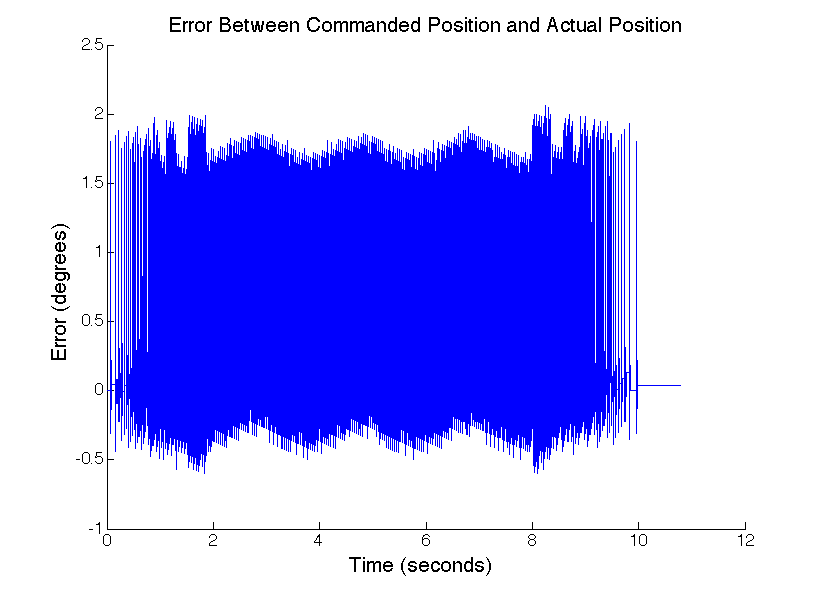
\includegraphics[width = 12cm]{labViewCommandError.png}
\caption{Error between commanded and actual position vs time}
\label{Q4a_Alt6}
\end{center}
\end{figure}

\begin{figure}
\begin{center}
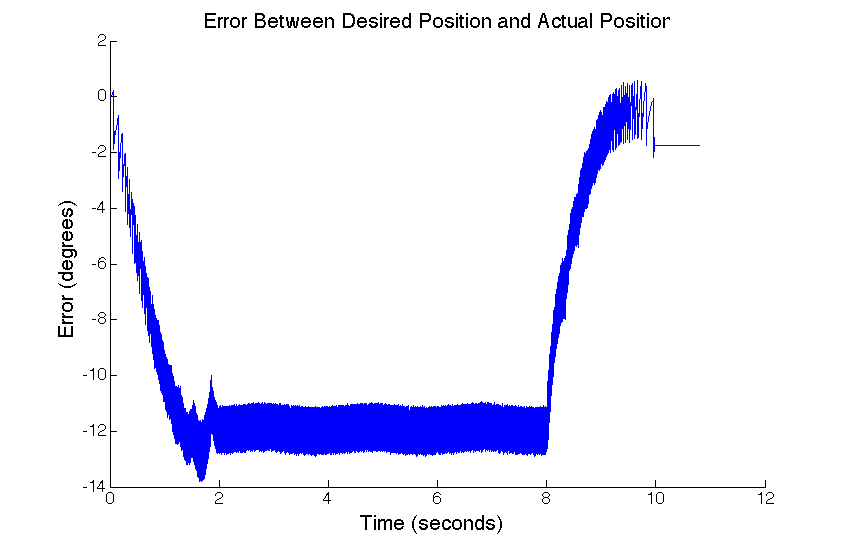
\includegraphics[width = 12cm]{labViewProfileError.png}
\caption{Error between desired position and actual position.}
\label{Q4a_Alt7}
\end{center}
\end{figure}

\clearpage

% end john's stuff
%%%%%%%%%%%%%%%%%%%%%%%

Considering the above concerns, the function generator was used to overcome the issues. Because the step command into the driver chip comes directly from the function generator, the pulse train could be generated with extremely high frequency, breaking through the frequency limit (1kHz; 500Hz step frequency) of LabView. Figure~\ref{fig:q4_5} and~\ref{fig:q4_6} show the VI front panel and block diagram used to accomplish various stepping modes including full, half, quarter and 1/8$^{th}$ steps.\\

The function generator used was an Agilent 33521A. To generate the trapezoidal profile for full steps with a constant speed region of 180 $deg/sec$ we used the following settings: square wave, sweep mode on, start frequency = 1mHz, stop frequency = 100Hz, sweep time = 2.0 sec, hold time = 6.0 sec, and return time = 2.0 sec. We then set the trigger to manual so that we could start the profile after the LabView VI was running. To change the step size while maintaining the same constant speed value, we kept the same time values while changing the stop frequency (for example, 800Hz for 1/8$^{th}$ stepping at 180 $deg/sec$) and changing the MS1 and MS2 settings within LabView. To change the value of the constant speed, we calculated the time required to turn 1080 degrees at the desired speed to get the hold time. Dividing 360 by the desired speed gave us the sweep and return times.\\

\begin{figure}[h!]
\begin{center}
%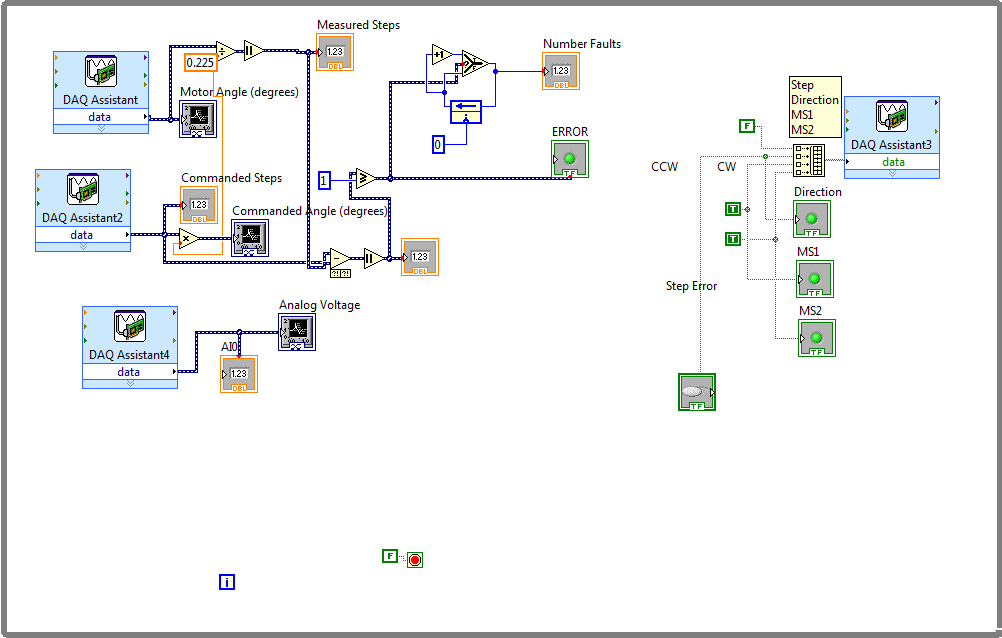
\includegraphics[width=16cm]{Q4_BlockDiagram_VI.png}
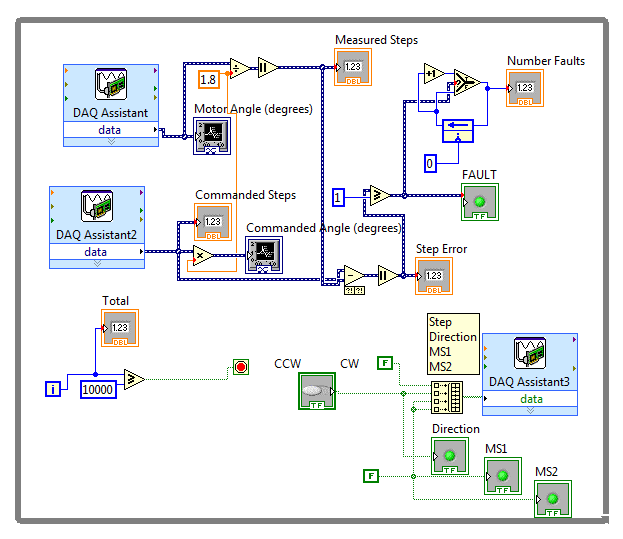
\includegraphics[width=16cm]{ExternalsourceBack.png}
\caption{Block Diagram of VI for Trapezoidal Velocity Profile Using Function Generator} \label{tex}
\label{fig:q4_5}
\end{center}
\end{figure}

\begin{figure}[h!]
\begin{center}
%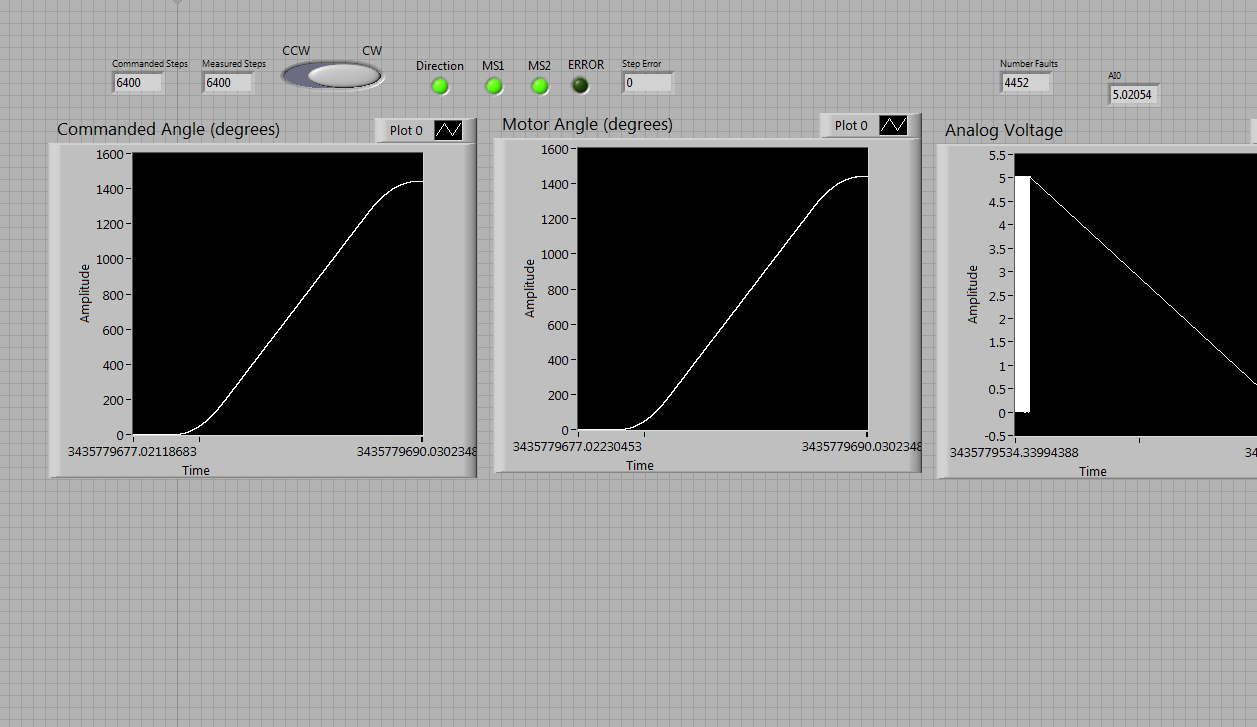
\includegraphics[width=12cm]{Q4_FrontPanel_VI.png}
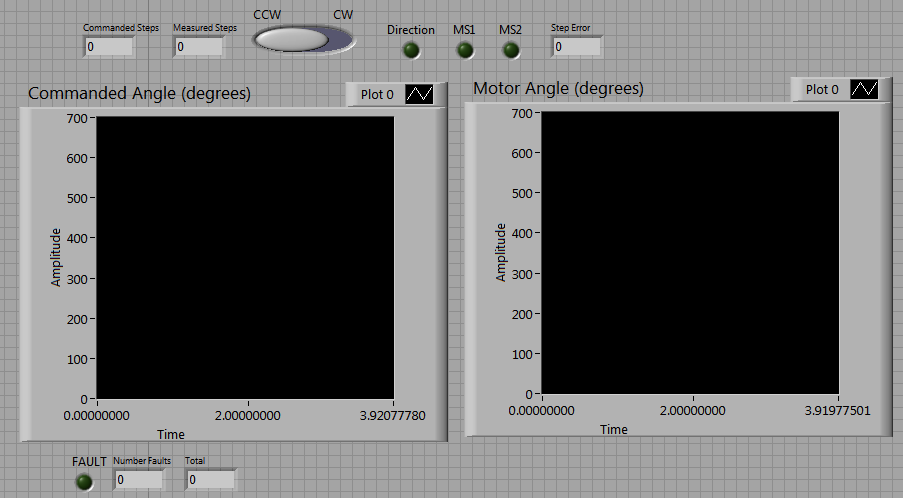
\includegraphics[width=12cm]{ExternalSourceFront.png}
\caption{Front Panel of VI for Trapezoidal Velocity Profile Using Function Generator} \label{tex}
\label{fig:q4_6}
\end{center}
\end{figure}

Figure~\ref{fig:q4_7},~\ref{fig:q4_8},~\ref{fig:q4_9} and Figure~\ref{fig:q4_10} show the command and actual displacement based on four stepping modes. As a whole, it seems only small difference between the reference and the real angular position. The total motion for any stepping mode is 1440deg read by the optical encoder, which is exactly the desired position. Figure~\ref{fig:q4_11},~\ref{fig:q4_12},~\ref{fig:q4_13} and Figure~\ref{fig:q4_14} show the velocity profiles estimated by the low-pass filter with $\tau$=0.25. The results suggest that as the increment step decreases, the amplitude of oscillations in the region of constant speed becomes smaller. All stepping modes met the criteria of total motion equal to 1440deg (as shown in figure \ref{fig:q4_9}), 1080deg of displacement during constant speed (see next paragraph), constant speed = 180 deg/sec (see figures \ref{fig:q4_11}, \ref{fig:q4_12}, \ref{fig:q4_13}, and \ref{fig:q4_14}), and oscillations of speed $<$5\% (see figures \ref{fig:q4_11}, \ref{fig:q4_12}, \ref{fig:q4_13}, and \ref{fig:q4_14}). \\

For the criterion that the region of constant speed should be at least 1080 deg, the results of various stepping modes are shown in Table~\ref{table:Q4_1}. The following are two steps to calculate the total displacement during the constant speed stage. First, determine the starting and end time of the constant speed region. Considering the rough estimation of velocity, the starting time was defined when the velocity began to reach \%95 of 180 deg/sec; the end time was defined when the velocity went down less than \%95 of 180 deg/sec. Second, once these times were known, we could find the corresponding displacement with respect to time, and the total displacement could be calculated. The results show that the displacement for all modes are close to 1080 deg. Even though some values are lower than 1080 deg which is the minimum requirement, this condition could be attributed to the inaccurate velocity estimation by the low-pass filter.   

\begin{table}[ht]
\caption{Estimation of Constant Speed Region} % title of Table
\centering  % used for centering table
\begin{tabular}{c c c c c}\\ % centered columns (5 columns)
\hline                        %inserts a horizontal line

 & Full & Half & Quarter & Eighth\\ [0.5ex] % inserts table 
%heading
\hline                  % inserts single horizontal line
Starting Time & 2.044 & 2.122 & 2.070 & 2.560 \\ % inserting body of the table
Ending Time & 7.962 & 8.103 & 8.059 & 8.567 \\
Starting Angle & 224.5 & 224.8 & 211.6 & 224.5 \\
Ending Angle & 1302 & 1302 & 1305 & 1303 \\
\hline \\%inserts single line
Total Displacement & 1077.5 & 1077.2 & 1093.4 & 1078.5\\[1ex]      % [1ex] adds vertical space

\hline %inserts single line
\end{tabular}
\label{table:Q4_1} % is used to refer this table in the text
\end{table}

\begin{figure}[hbt]
\begin{center}
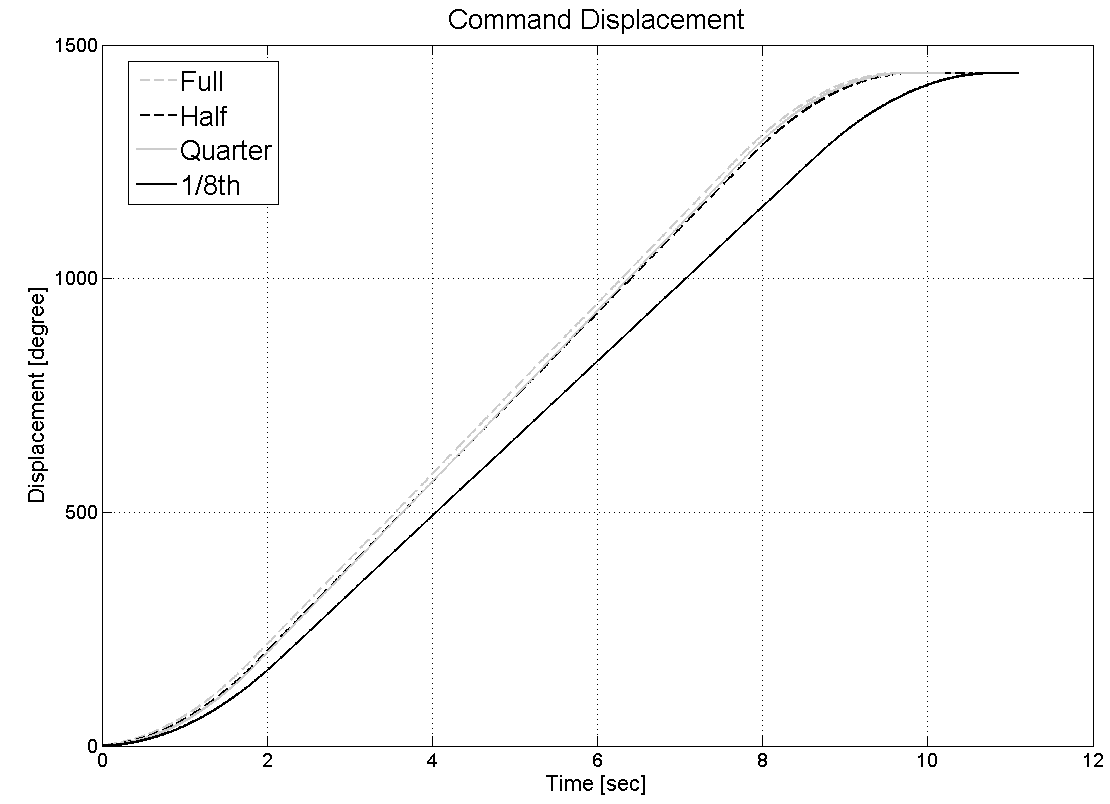
\includegraphics[width=12cm]{Q4_CommandPosition.png}
\caption{Command Displacement vs. Time} \label{tex}
\label{fig:q4_7}
\end{center}
\end{figure}

\begin{figure}[hbt]
\begin{center}
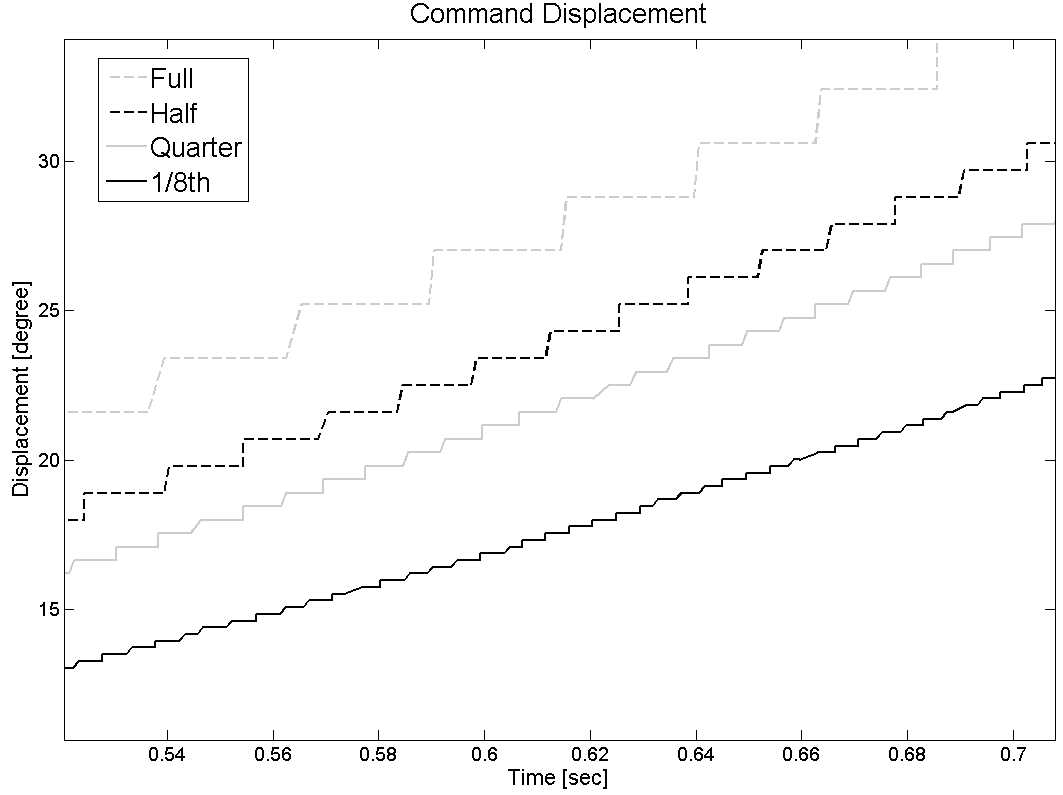
\includegraphics[width=12cm]{Q4_CommandPosition_L.png}
\caption{Command Displacement vs. Time (Zoom In)} \label{tex}
\label{fig:q4_8}
\end{center}
\end{figure}

\begin{figure}[h]
\begin{center}
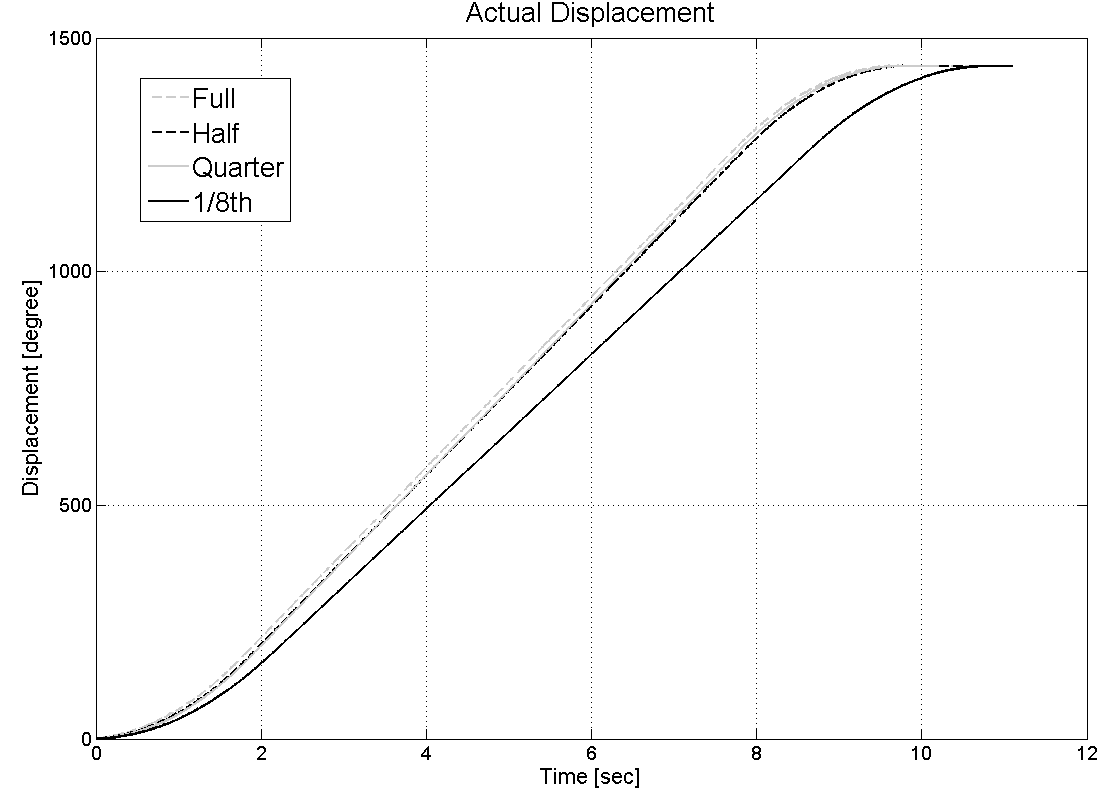
\includegraphics[width=12cm]{Q4_ActualPosition.png}
\caption{Actual Displacement vs. Time - All step modes reach 1440deg} \label{tex}
\label{fig:q4_9}
\end{center}
\end{figure}

\begin{figure}[h]
\begin{center}
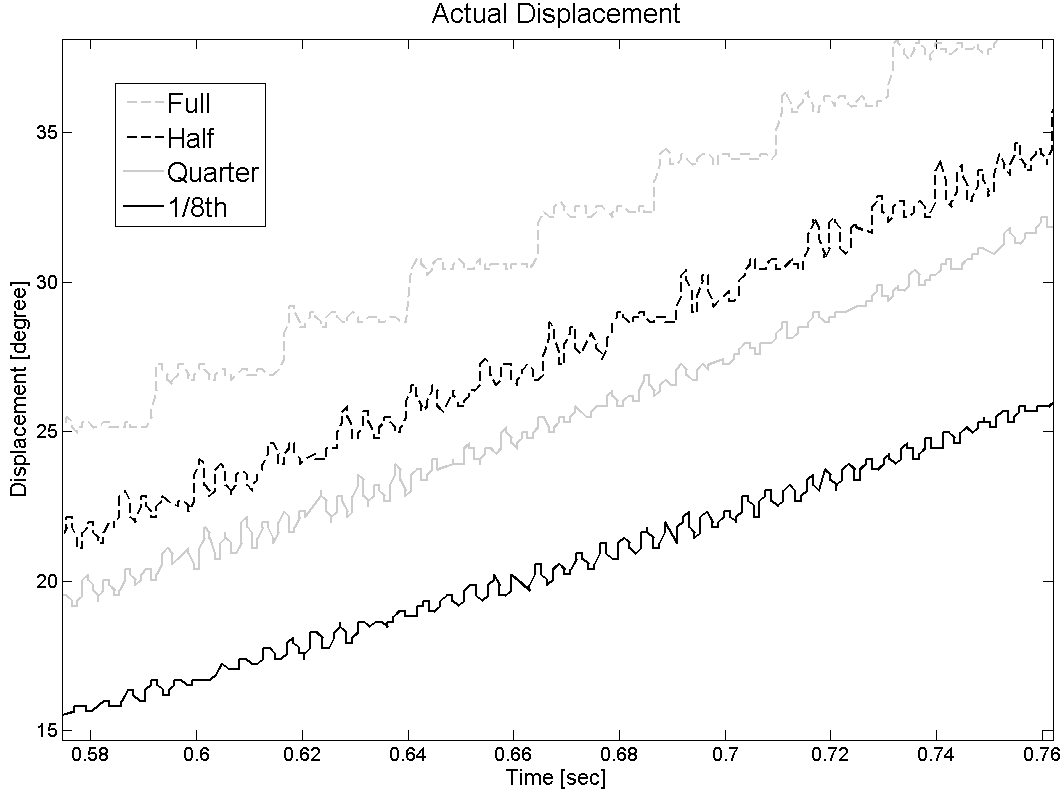
\includegraphics[width=12cm]{Q4_ActualPosition_L.png}
\caption{Actual Displacement vs. Time (Zoom In)} \label{tex}
\label{fig:q4_10}
\end{center}
\end{figure}

\begin{figure}[h!]
\begin{center}
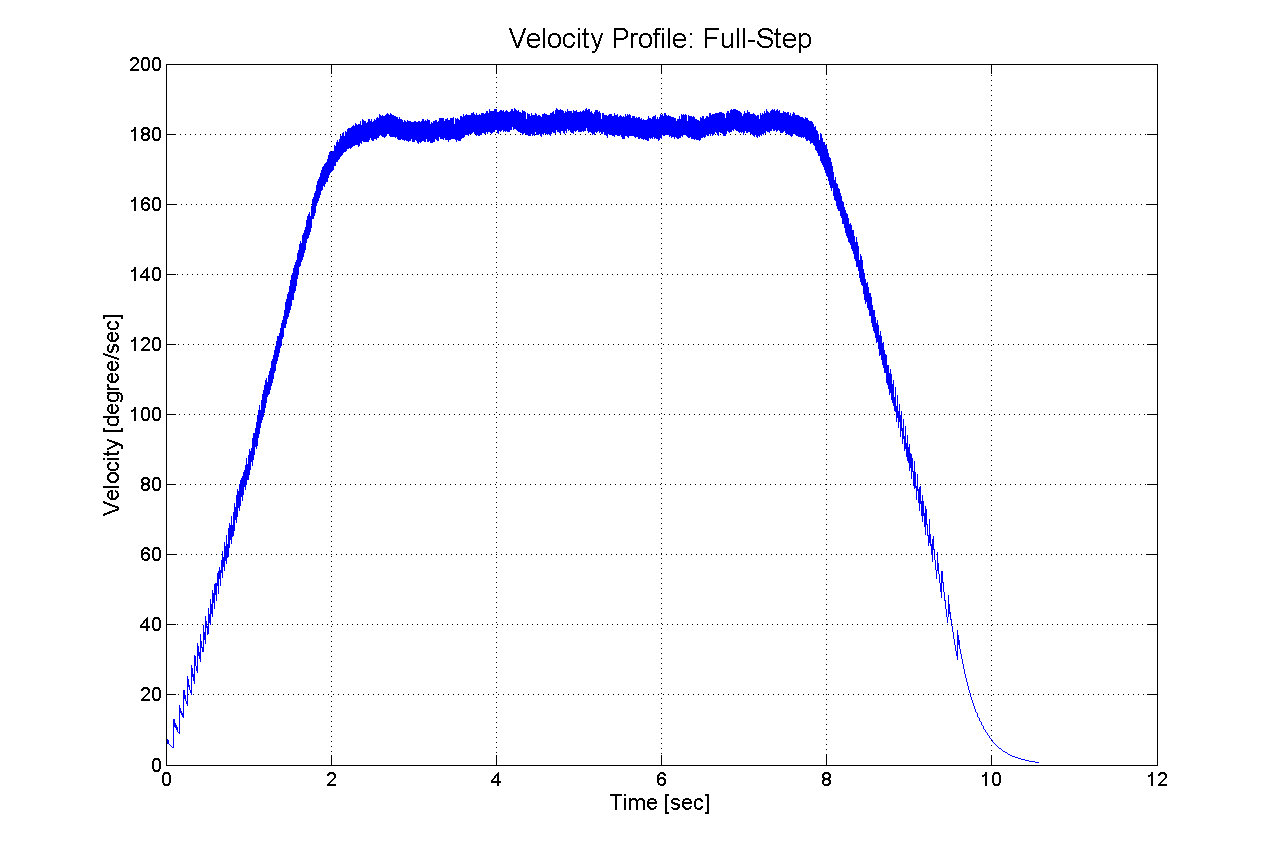
\includegraphics[width=12cm]{Q4_full_step.png}
\caption{Velocity Profile: Full-Step Mode - Constant velocity within 5\% of 180deg/sec} \label{tex}
\label{fig:q4_11}
\end{center}
\end{figure}

\begin{figure}[h!]
\begin{center}
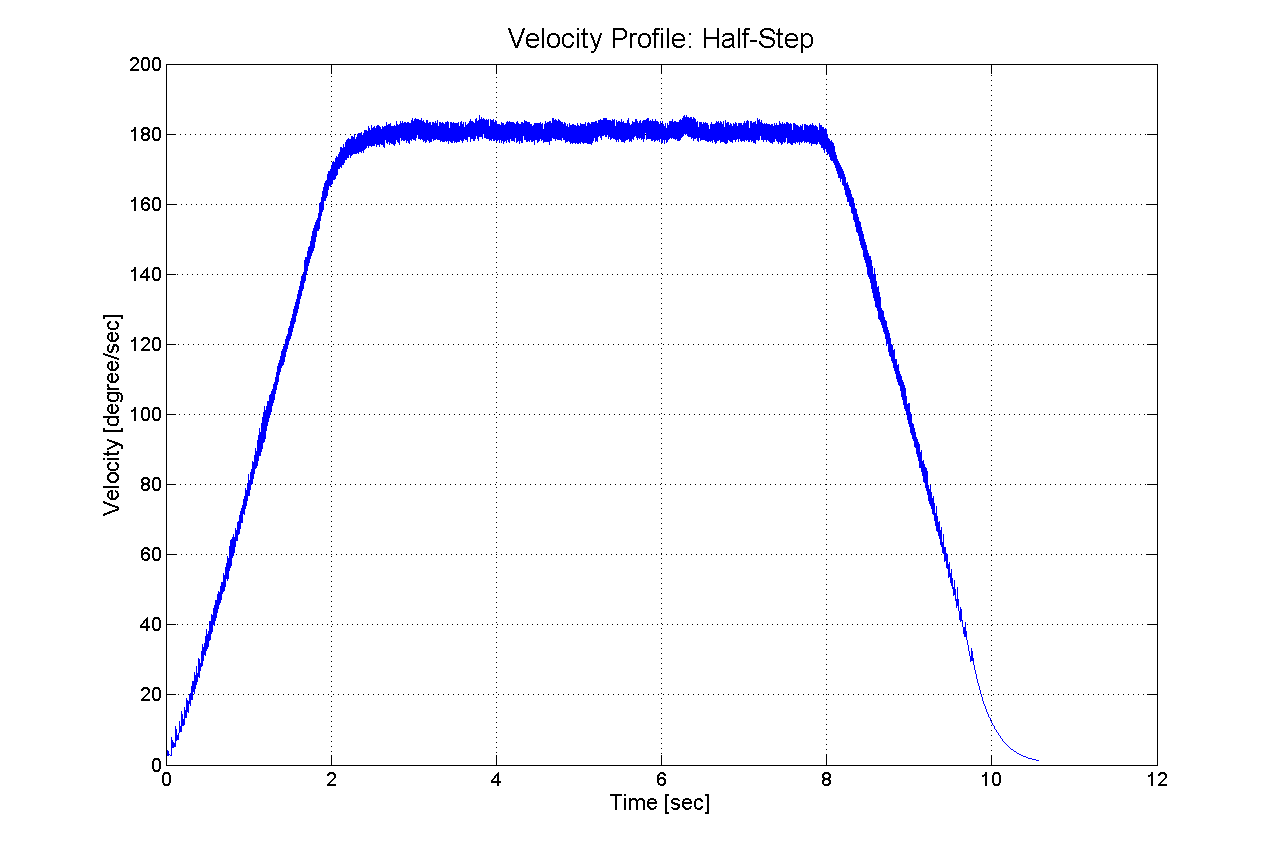
\includegraphics[width=12cm]{Q4_half_step.png}
\caption{Velocity Profile: Half-Step Mode - Constant velocity within 5\% of 180deg/sec} \label{tex}
\label{fig:q4_12}
\end{center}
\end{figure}

\begin{figure}[h!]
\begin{center}
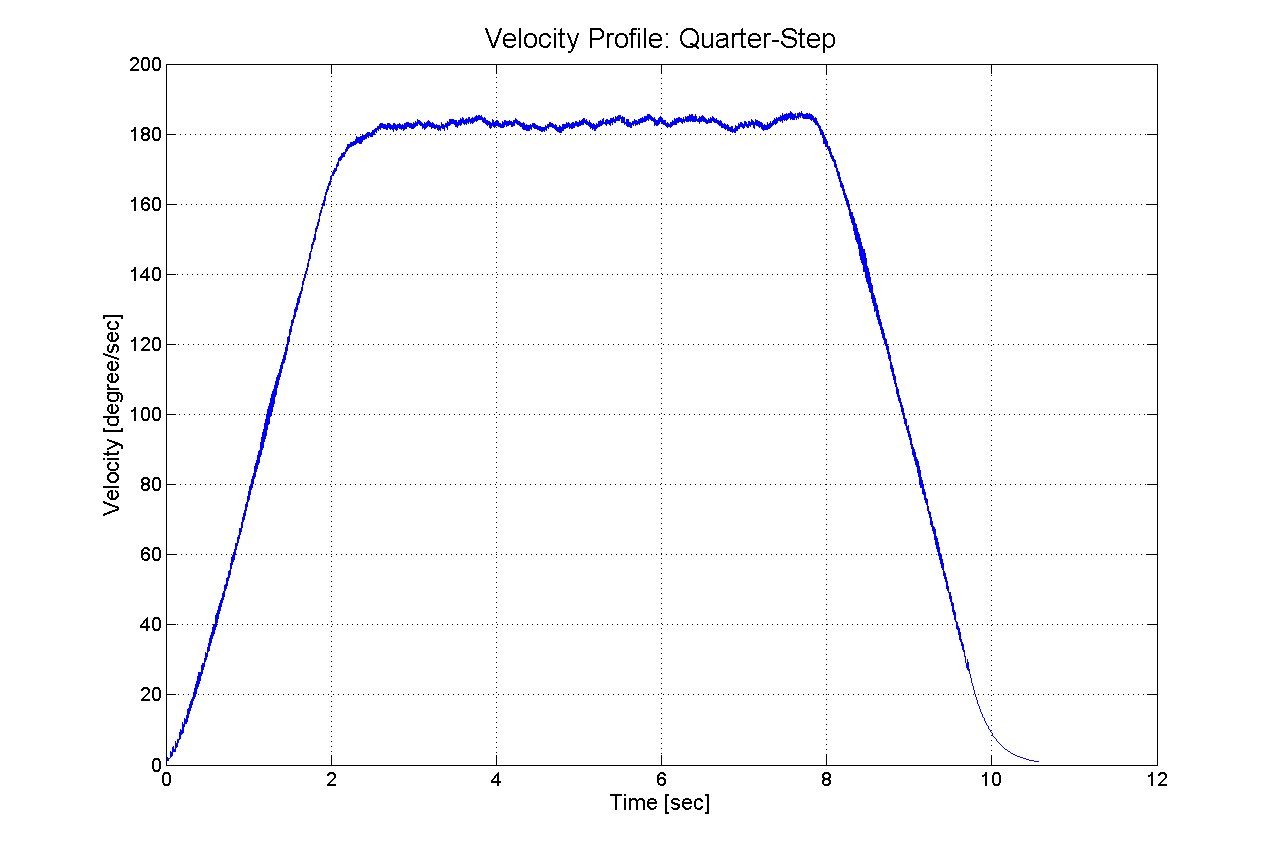
\includegraphics[width=12cm]{Q4_quarter_step.png}
\caption{Velocity Profile: Quarter-Step Mode - Constant velocity within 5\% of 180deg/sec} \label{tex}
\label{fig:q4_13}
\end{center}
\end{figure}

\begin{figure}[h!]
\begin{center}
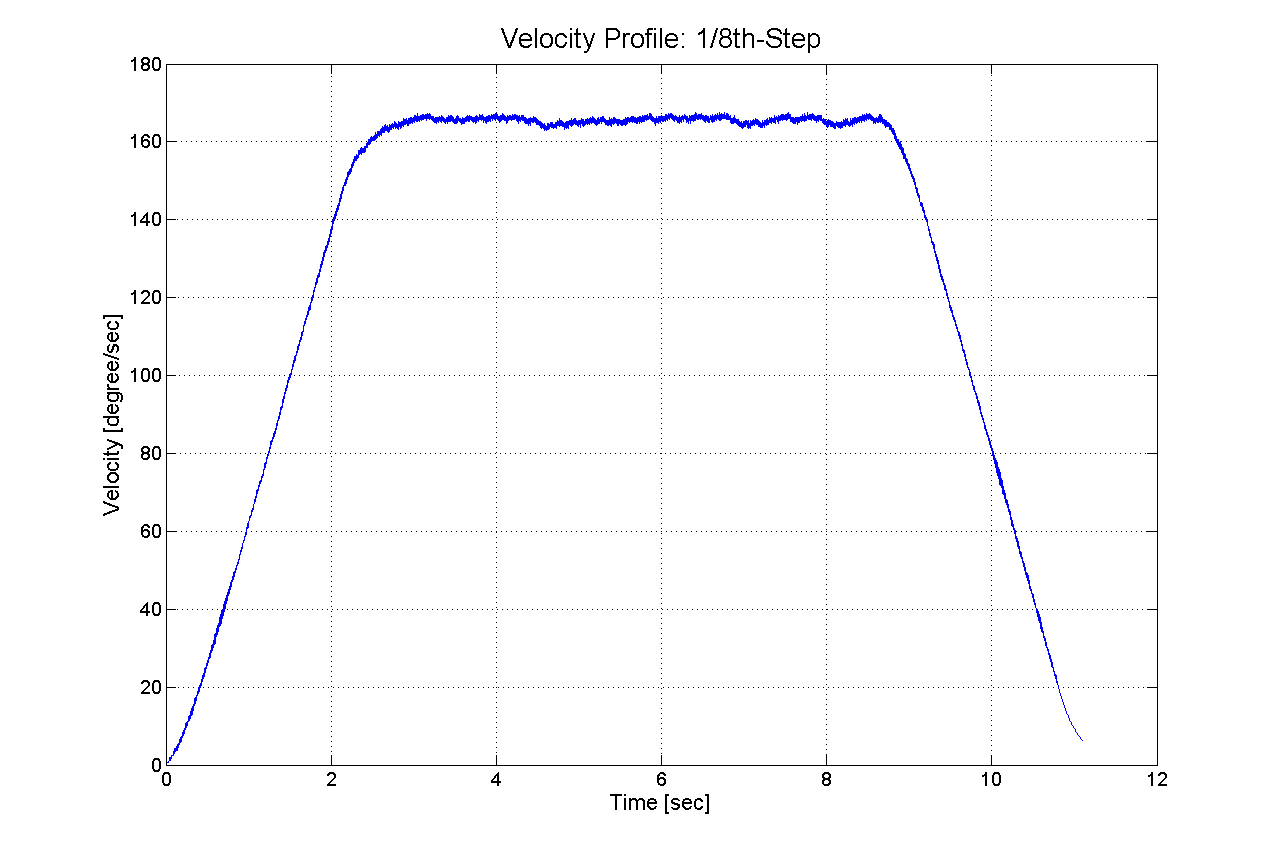
\includegraphics[width=12cm]{Q4_eighth_step.png}
\caption{Velocity Profile: 1/8-Step Mode - Constant velocity within 5\% of 180deg/sec} \label{tex}
\label{fig:q4_14}
\end{center}
\end{figure}

\clearpage

\subsection*{b.}

As can be seen in Figure~\ref{fig:q4_10} on page \pageref{fig:q4_10}, the smaller increment step provides greater resolution and smoother motor operation, i.e. smoother velocity and displacement, while the undesired behavior of overshoot seems to become more serious. Since the resolution of the optical encoder is relatively low compared the increment step, the real profiles for all modes are expected to be smoother. Figure~\ref{fig:q4_15},~\ref{fig:q4_16},~\ref{fig:q4_17} and Figure~\ref{fig:q4_18} (on pages \pageref{fig:q4_15},\pageref{fig:q4_16},\pageref{fig:q4_17} and \pageref{fig:q4_18} respectively) show the details of profile comparison between the command and actual displacement. We can observe that the overshoot in the full-step mode is less than 50\%, while approximately 100\% overshoot occurs in the half-step mode. For the quarter and 1/8 stepping modes, the oscillation behavior is hardly observed because of the low resolution. We were not able to implement half or quarter stepping using LabView due to the limitations on frequency outputs, but we were able to achieve up to 1/8$^{th}$ stepping with the function generator. \\

\begin{figure}[htb]
\begin{center}
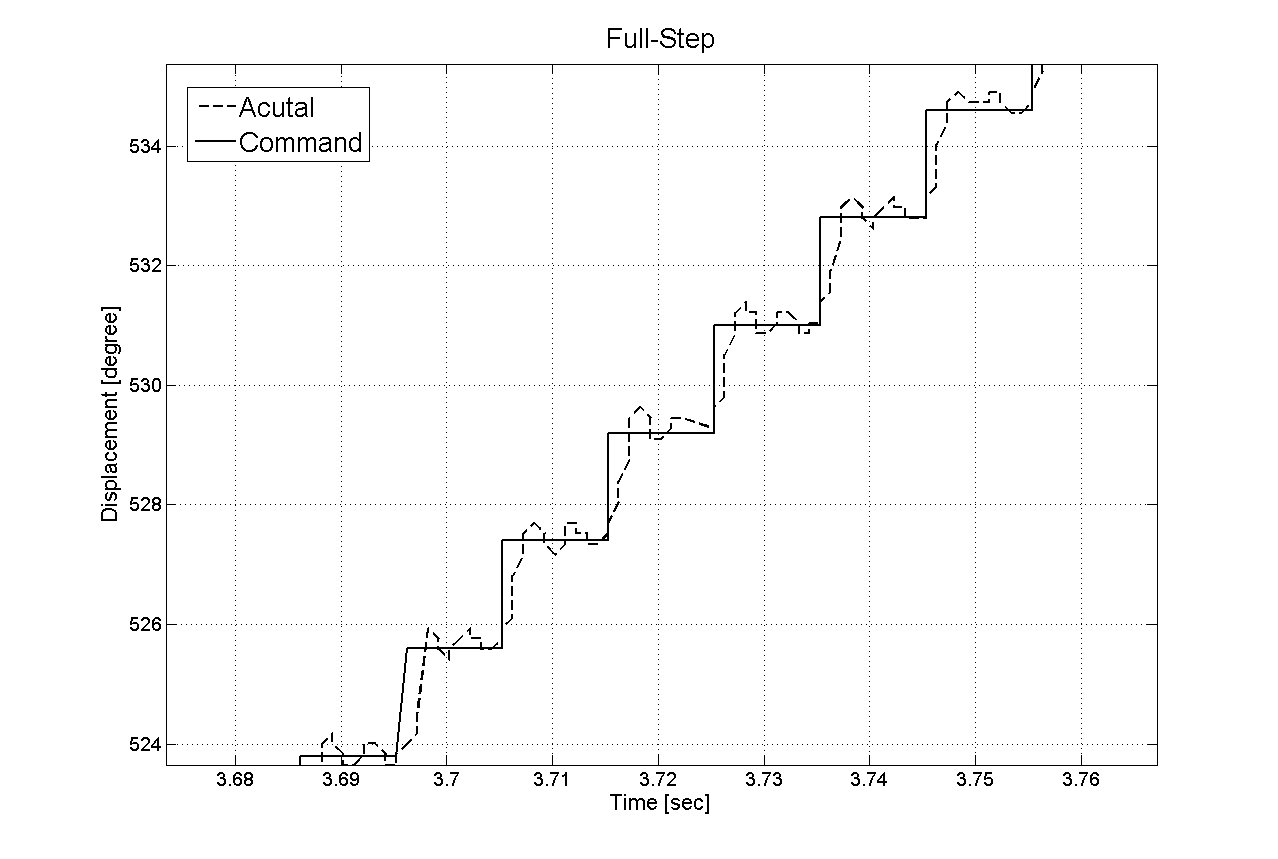
\includegraphics[width=14cm]{Q4_full_step_L.png}
\caption{Full-Step: Command vs. Actual Displacement} \label{tex}
\label{fig:q4_15}
\end{center}
\end{figure}

\begin{figure}[htb]
\begin{center}
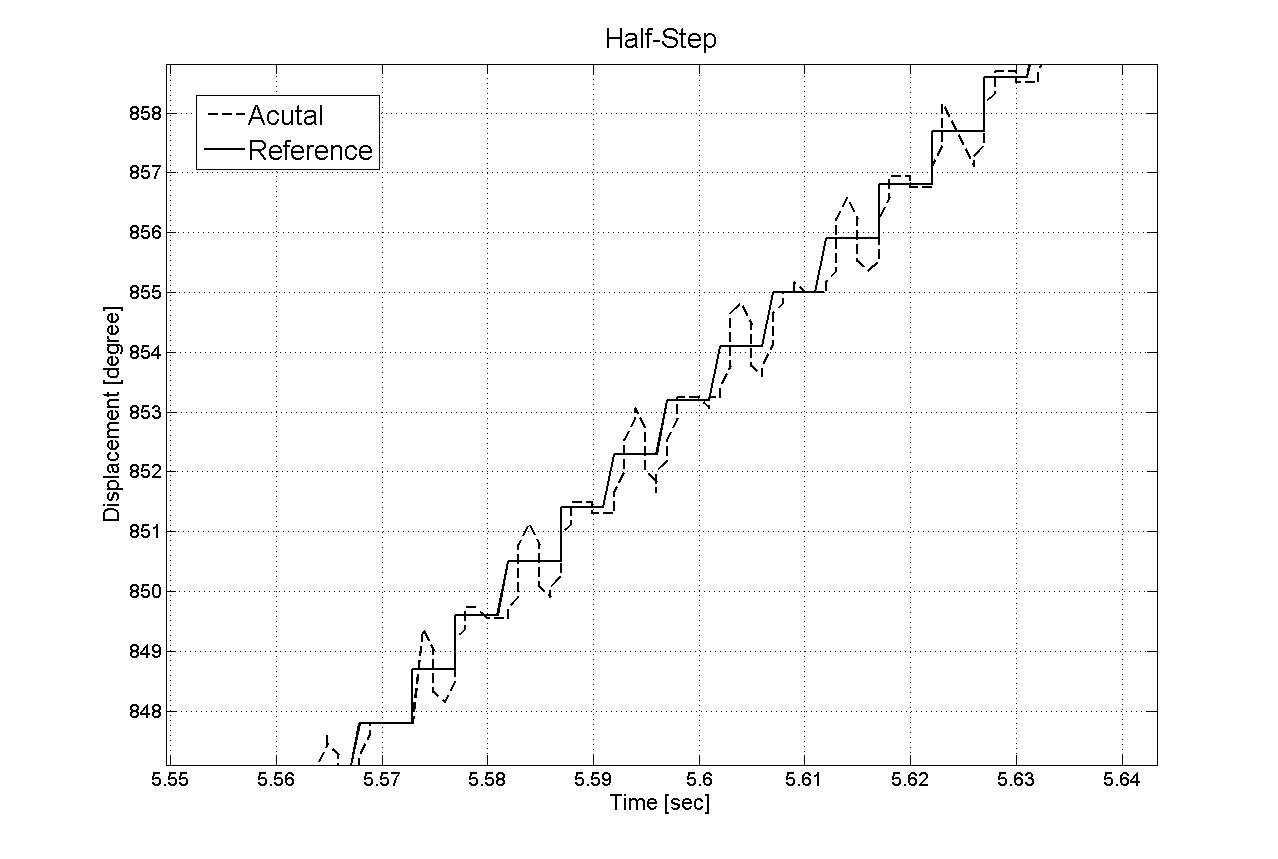
\includegraphics[width=14cm]{Q4_half_step_L.png}
\caption{Half-Step: Command vs. Actual Displacement} \label{tex}
\label{fig:q4_16}
\end{center}
\end{figure}


\begin{figure}[htb]
\begin{center}
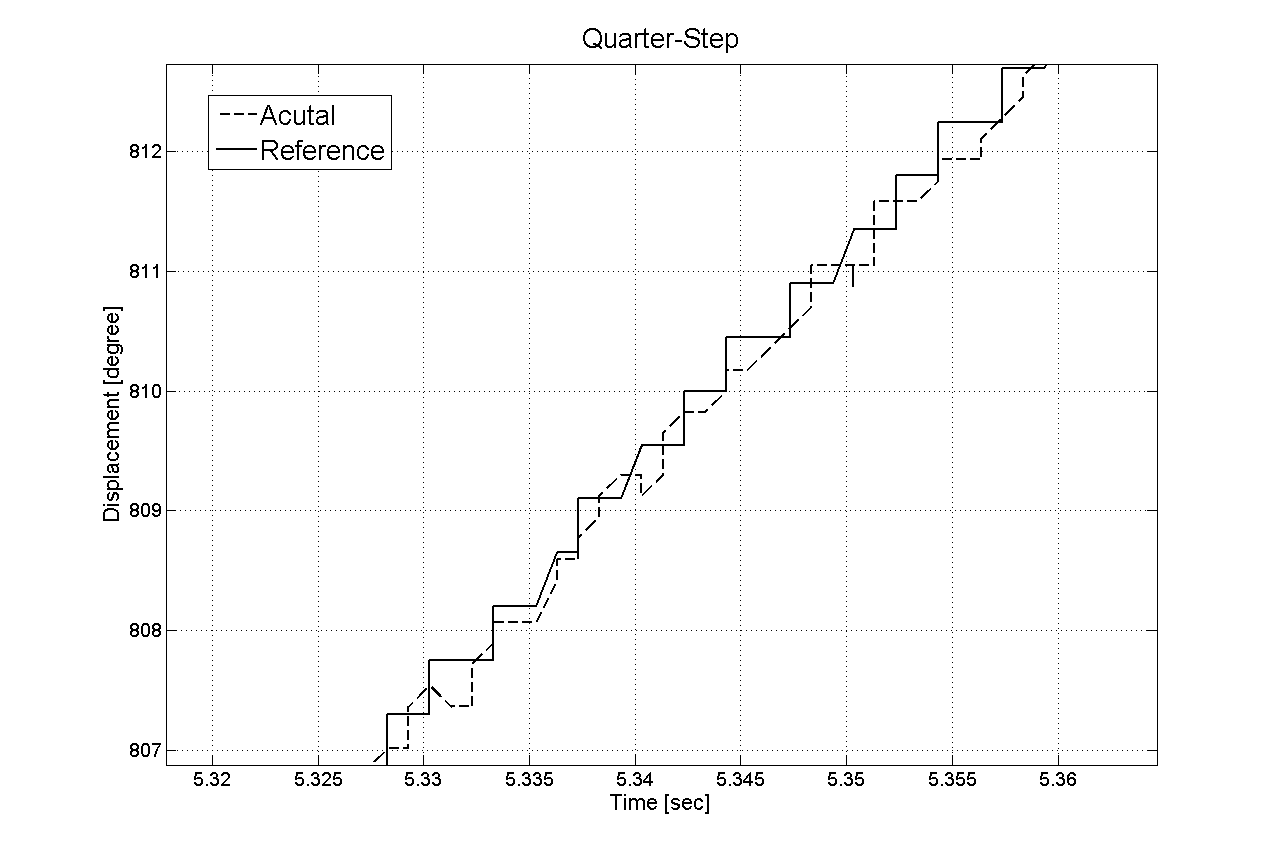
\includegraphics[width=14cm]{Q4_quarter_step_L.png}
\caption{Quarter-Step: Command vs. Actual Displacement} \label{tex}
\label{fig:q4_17}
\end{center}
\end{figure}

\begin{figure}[htb]
\begin{center}
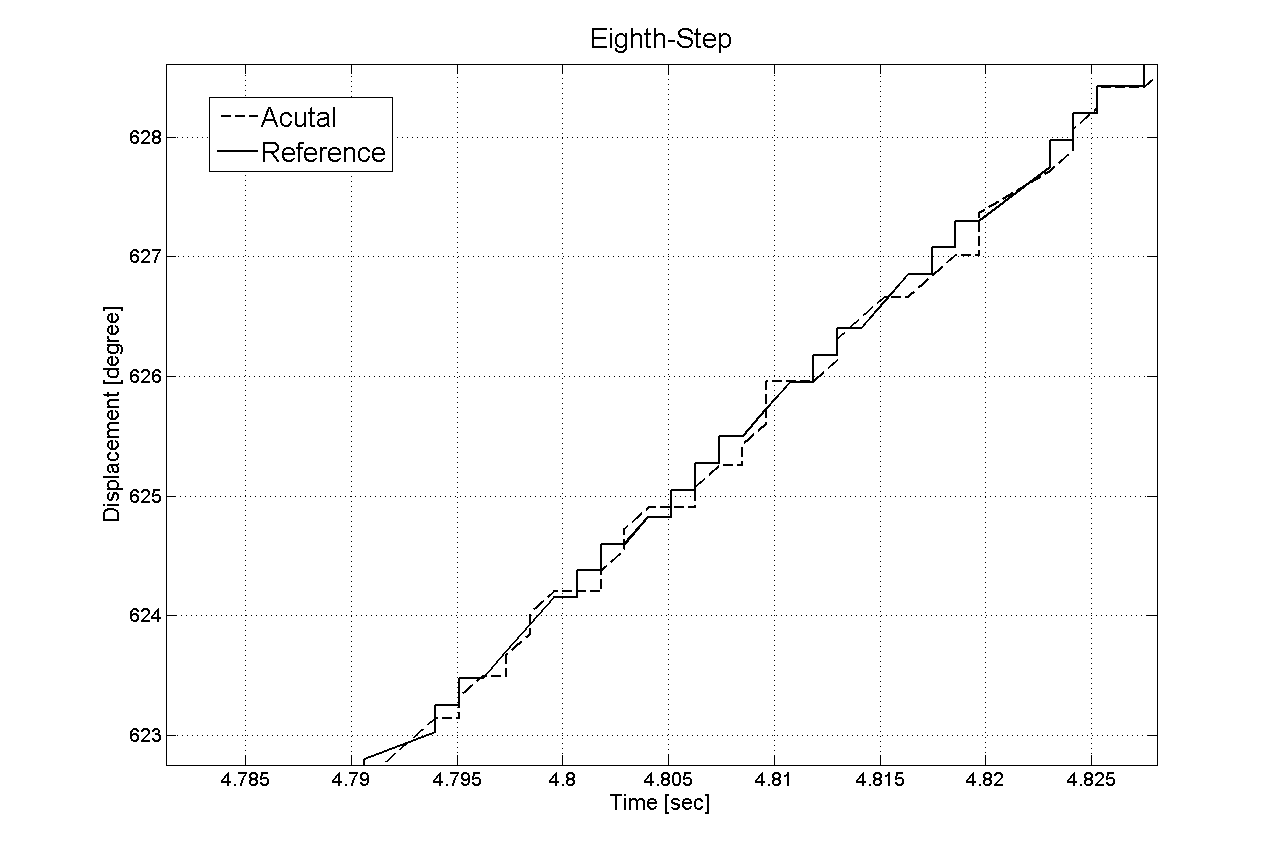
\includegraphics[width=14cm]{Q4_eighth_step_L.png}
\caption{1/8-Step: Command vs. Actual Displacement} \label{tex}
\label{fig:q4_18}
\end{center}
\end{figure}

\clearpage 


\subsection*{c.}

We were able to achieve angular velocities up to $1939.7 \, \sfrac{deg}{s}$ using the function generator while meeting all of the constraints.  This maximum speed was limited only by the pull-out speed of the stepper motor.  As shown in figure \ref{Q4c_ProfileDetail}, on  page \pageref{Q4c_ProfileDetail}, a substantial amount of the error between the desired angular position and actual angular position seen in figure ~\ref{Q4c_PE}, on page \pageref{Q4c_PE}, is due to the dynamics of the stepper motor and its discrete positions.  We also see a difference between the commanded position and the desired position, shown in figure \ref{Q4c_CE}, on page \pageref{Q4c_CE}, which is due to the discrete nature of the position commands issued to the stepper motor.  Using a finer step setting on the driver would reduce this error.\\

\begin{figure}[hbt]
\begin{center}
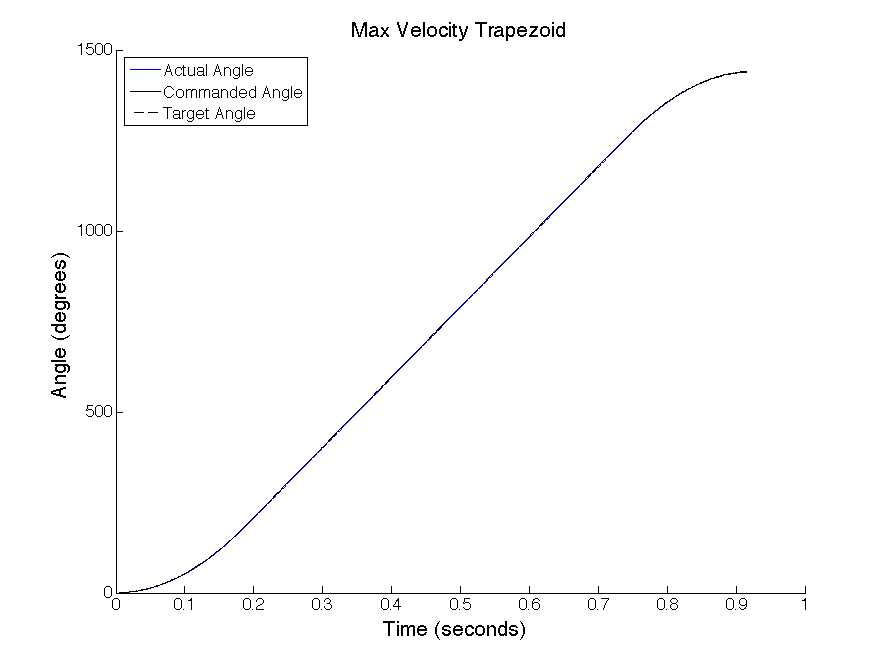
\includegraphics[width = 12cm]{4cProfile.png}
\caption{Commanded Profile vs Recorded Position vs Target Position}
\label{Q4c_Profile}
\end{center}
\end{figure}

\begin{figure}[hbt]
\begin{center}
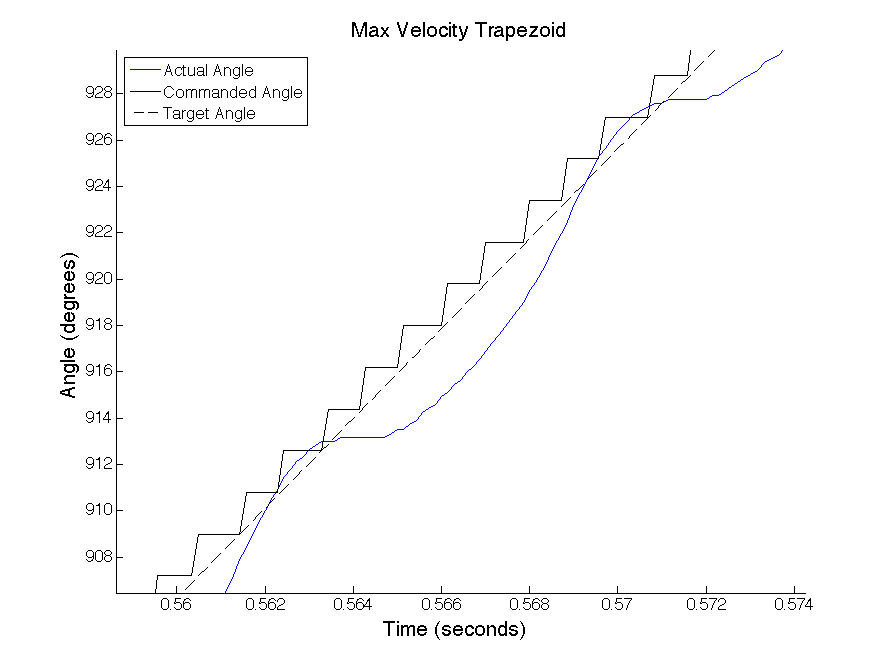
\includegraphics[width = 12cm]{4cProfileDetail1.png}
\caption{Commanded Profile vs Recorded Position vs Desired Position}
\label{Q4c_ProfileDetail}
\end{center}
\end{figure}

\begin{figure}[hbt]
\begin{center}
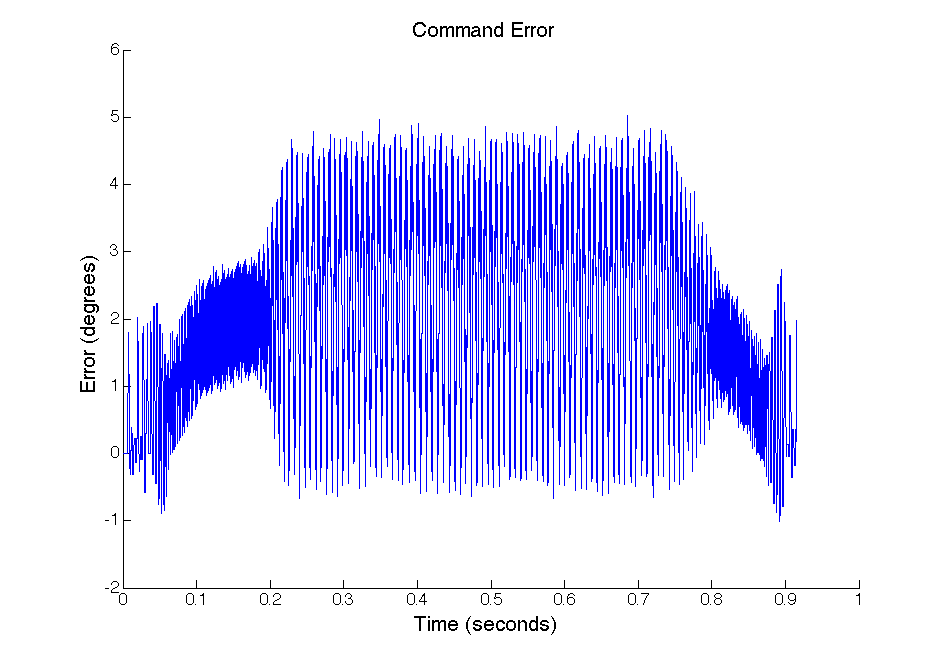
\includegraphics[width = 12cm]{4cCommandError.png}
\caption{Error between Commanded Profile and Desired Profile}
\label{Q4c_CE}
\end{center}
\end{figure}

\begin{figure}[hbt]
\begin{center}
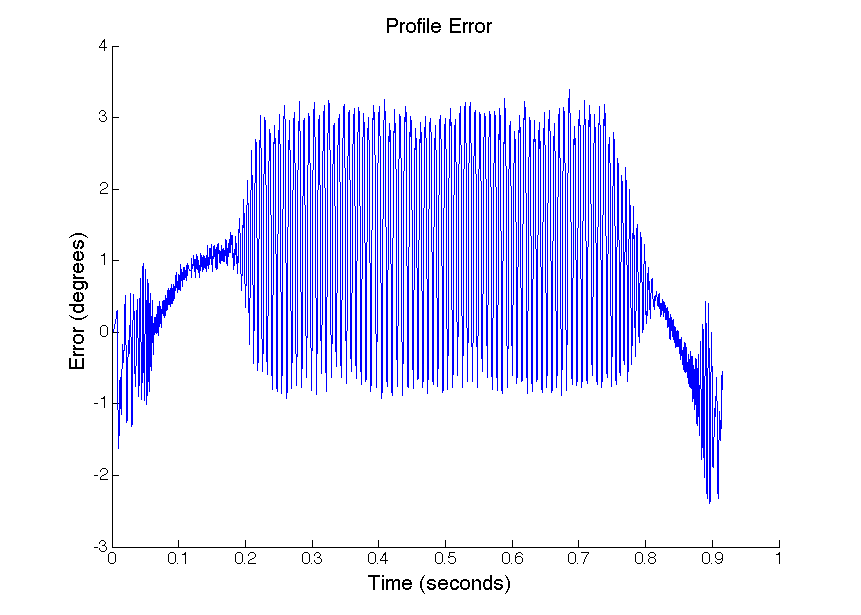
\includegraphics[width = 12cm]{4cProfileError.png}
\caption{Error between Desired Profile and Actual Profile}
\label{Q4c_PE}
\end{center}
\end{figure}

\clearpage




%\clearpage
%\section*{Appendix.}

%\subsection*{System Energy Computation}
%\xxx{Uncomment below to add m-file code}
%\verbatiminput{totalEnergy.m}

\end{document}